\chapter{涵道风扇式无人机的控制分配}
由涵道无人机的非线性数学模型\eqref{eq_nonlinear_model}可知,该系统需要控制六个自由度但操纵面只有四个,因而该系统是一个欠驱动系统。但对于姿态子系统而言,被控量变为三自由度的旋转运动,操纵面数大于被控量自由度,因此姿态子系统是过驱动系统。过驱动系统的控制分配解决的是如何将控制量映射到冗余配置的操纵面(或执行器),使操纵面产生的控制效应等于或者尽可能接近于期望的控制量。该控制量又称伪控制输入或虚拟控制,其物理意义通常是力或者力矩,亦或是力和力矩的组合,因而又称广义力矩。本章先介绍控制分配基础,再别分析单涵道和双涵道的控制分配问题,并给出求解方法。
\section{控制分配基础}
%
\subsection{控制分配问题}
%
引入伪控制输入后,过驱动系统可以用如下所示的两个子系统描述
\begin{align}
&\left\{\begin{array}{l}
\dot{\bm{x}}= \bm{f}\left( \bm{x} \right) + \bm{G} \bm{\tau} \\
\bm{y} = \bm{h}\left( \bm{x} \right)
\end{array}\right. \label{eq_intro_v_sys}	\\
%\end{align}
%\begin{align}
&\left\{\begin{array}{l}
\dot{\bm{x}}_{\delta}  = \bm{f}_{\delta} \left( \bm{x}_{\delta},\bm{\delta}_c \right)  \\
\bm{\delta}=h_{\delta}\left( \bm{x}_{\delta} \right) 
\end{array}\right. \label{eq_atuacor}
\end{align}
其中式\eqref{eq_intro_v_sys}为被控过程的动力学模型$\bm{x}\in {\mathbb{R}}^{\text{n}}$为过程状态,如飞行器状态,$\bm{\tau}$表示伪控制输入,$\bm{y} \in \mathbb{R}^{m}$为系统输出,${\bm{\delta}}\in{\bm{\Omega}}\subset\mathbb{R}^{p}$ 为操纵面偏转角,同时是执行器的输出,$\bm{G}\in {\mathbb{R}}^{\text{m}}$,映射$\bm{f}: \mathbb{R}^{n} \rightarrow \mathbb{R}^{n}$,$\bm{g}: \mathbb{R}^{n} \times \mathbb{R}^{p} \rightarrow \mathbb{R}^{n}$,$\bm{h}: \mathbb{R}^{n} \rightarrow \mathbb{R}^{m}$。式\eqref{eq_atuacor}为执行器动力学模型,其中$\bm{x}_{\delta} \in \mathbb{R}^{q} $为执行器状态,${\bm{\delta}_c} \in {\bm{\Omega}}$ 为执行器指令,是整个系统的控制输入,又称为控制向量。映射$\bm{f}_{\delta}: \mathbb{R}^{q} \rightarrow \mathbb{R}^{q}$,$\bm{h}_{\delta}: \mathbb{R}^{q} \rightarrow \mathbb{R}^{p}$。为简单起见,假定系统输出的维数即为系统的自由度,$\bm{\tau}\in \bm{\Phi} \subset \mathbb{R}^{m}$,对过驱动系统有$m<p$。设操纵面模型为
\begin{align}
\bm{\tau} =\bm{M}(\bm{x}, \bm{\delta})  \label{eq_effetor_model}
\end{align}
其中,映射$\bm{M}: \mathbb{R}^{n} \times \mathbb{R}^{p} \rightarrow \mathbb{R}^{m}$,伪控制输入通常为$m$维广义力或力矩,在本文中统一称$\bm{\tau}$为力矩。

由于操纵面存在约束,$\bm{\Omega}$是$\mathbb{R}^{p}$的子集,称为容许控制集,属于$\bm{\Omega}$的$\bm{\delta}$称为容许控制。容许控制集通过$\bm{M}$从$\mathbb{R}^{p}$空间映射到$\mathbb{R}^{m}$空间得到系统的可达力矩集$\bm{\Phi}$,若$\bm{\tau}\in \bm{\Phi} $则称$\bm{\tau}$可达(Attainable)。

引入伪控制输入后,控制系统的设计可分为两步:首先由上层控制算法针对式\eqref{eq_intro_v_sys}设计的控制律${\bm{\tau}_c} \in {{\mathbb{R}}^m}$,然后控制分配环节将$\bm{\tau}_c$作为期望力矩,对给定$\bm{\tau}_c$,根据式\eqref{eq_effetor_model}、式\eqref{eq_atuacor}求解控制输入${\bm{\delta}_c} \in {\bm{\Omega}}$,使得$ \bm{\tau} $尽可能接近${\bm{\tau}_c}$。注意到,使式\eqref{eq_intro_v_sys}渐近稳定的控制律 不一定可达。

实际中更实用的是线性化的操纵面模型。当操纵面偏转角$\bm{\delta}$为零向量时称为零偏转,记为$\bm{\delta}_0$,将式\eqref{eq_effetor_model}在某系统状态下在$\bm{\delta}_0$处做泰勒展开
\begin{gather}
\bm{\tau} =\bm{B}\left(\bm{\delta}-\bm{\delta}_{0}\right)+\bm{\tau}_{0} \label{eq_tayler} \\
\bm{\tau}_{0} \triangleq \bm{M}\left(\bm{x}, \bm{\delta}_{0}\right) \\
\bm{B} \triangleq \dfrac{\partial \bm{\tau}}{\partial \bm{\delta}}=\left[\begin{array}{cccc}
\dfrac{\partial \tau_{1}}{\partial \delta_{1}} & \dfrac{\partial \tau_{1}}{\partial \delta_{2}} & \cdots & \dfrac{\partial \tau_{1}}{\partial \delta_{p}} \\
\dfrac{\partial \tau_{2}}{\partial \delta_{1}} & \dfrac{\partial \tau_{2}}{\partial \delta_{2}} & \cdots & \dfrac{\partial \tau_{2}}{\partial \delta_{p}} \\
\vdots & \vdots & \ddots & \vdots \\
\dfrac{\partial \tau_{m}}{\partial \delta_{1}} & \dfrac{\partial \tau_{m}}{\partial \delta_{2}} & \cdots & \dfrac{\partial \tau_{m}}{\partial \delta_{p}}
\end{array}\right]
\end{gather}
其中$\bm{B}\in {{\mathbb{R}}^{m\times p}}$称为控制效率矩阵,$\bm{B}$、$\bm{\tau}_{0}$都与系统状态相关。零偏转是认为定义的\cite{Durham_2017},$\bm{\delta}_0$还可以取为使$\bm{\tau}_{0}$为零向量时的操纵面偏转角。另外在具体实现中,控制系统以较高的频率运行,$\bm{\delta}_0$也可以取为上一采样时刻的值,因此式\eqref{eq_tayler}相当于将式\eqref{eq_effetor_model}在上一采样时刻做泰勒展开。通常将曲线$\bm{M}(\bm{x}, \bm{\delta}) $的离散数据存在计算机中,通过查表可求得曲线斜率进而求得$\bm{B}$,即使$\bm{\tau}_{0}$不为零向量时同样可以查表获得。将式\eqref{eq_tayler}改写为
\begin{align}
\bm{\tau}=\bm{B}\bm{\delta}+ \bm{\eta}
\end{align}
其中$ \bm{\eta}=\bm{\tau}_{0}-\bm{B}\bm{\delta}_{0} $称为截距项。重定义伪控制输入为$\bm{\tau} = \bm{\tau}_c-\bm{\eta}$,得到线性操纵面模型
\begin{align}
\bm{\tau}=\bm{B\delta} \label{eq_linear_model}
\end{align}
并基于式\eqref{eq_linear_model}讨论控制分配问题。

另一方面,控制分配算法求解得$\bm{\delta}_c$后,将作为执行器的指令,执行器使操纵面跟踪该指令。这部分通常集成在一些机电设备中,如无人直升机中所用的力矩舵机。相比于被控对象,通常执行器的动态响应时间非常短,因此在控制分配中通常假设操纵面偏转角等于执行器指令,即忽略执行器动态\eqref{eq_atuacor},有$\bm{\delta}=\bm{\delta}_c$,并且在控制分配中不做区分,统一记为$ \bm{\delta} $,并统一称为控制输入。

经过上述线性化以及忽略执行器动态的简化之后,控制分配问题描述为:对给定$\bm{\tau}= \bm{\tau}_c-\bm{\eta}$、$\bm{B}$及$\bm{\Omega}$,求$\bm{\delta}$,使得$\bm{\tau}=\bm{B}\bm{\delta}$且$\bm{\delta} \in \bm{\Omega}$。显然,对过驱动系统,式\eqref{eq_linear_model}是一个欠定方程,已知$ \bm{\tau} $求解$ \bm{\delta } $将出现多解。引入控制分配环节后,闭环控制系统如图\ref{fig_system}所示。
\begin{figure}[htbp]
	\centering	
	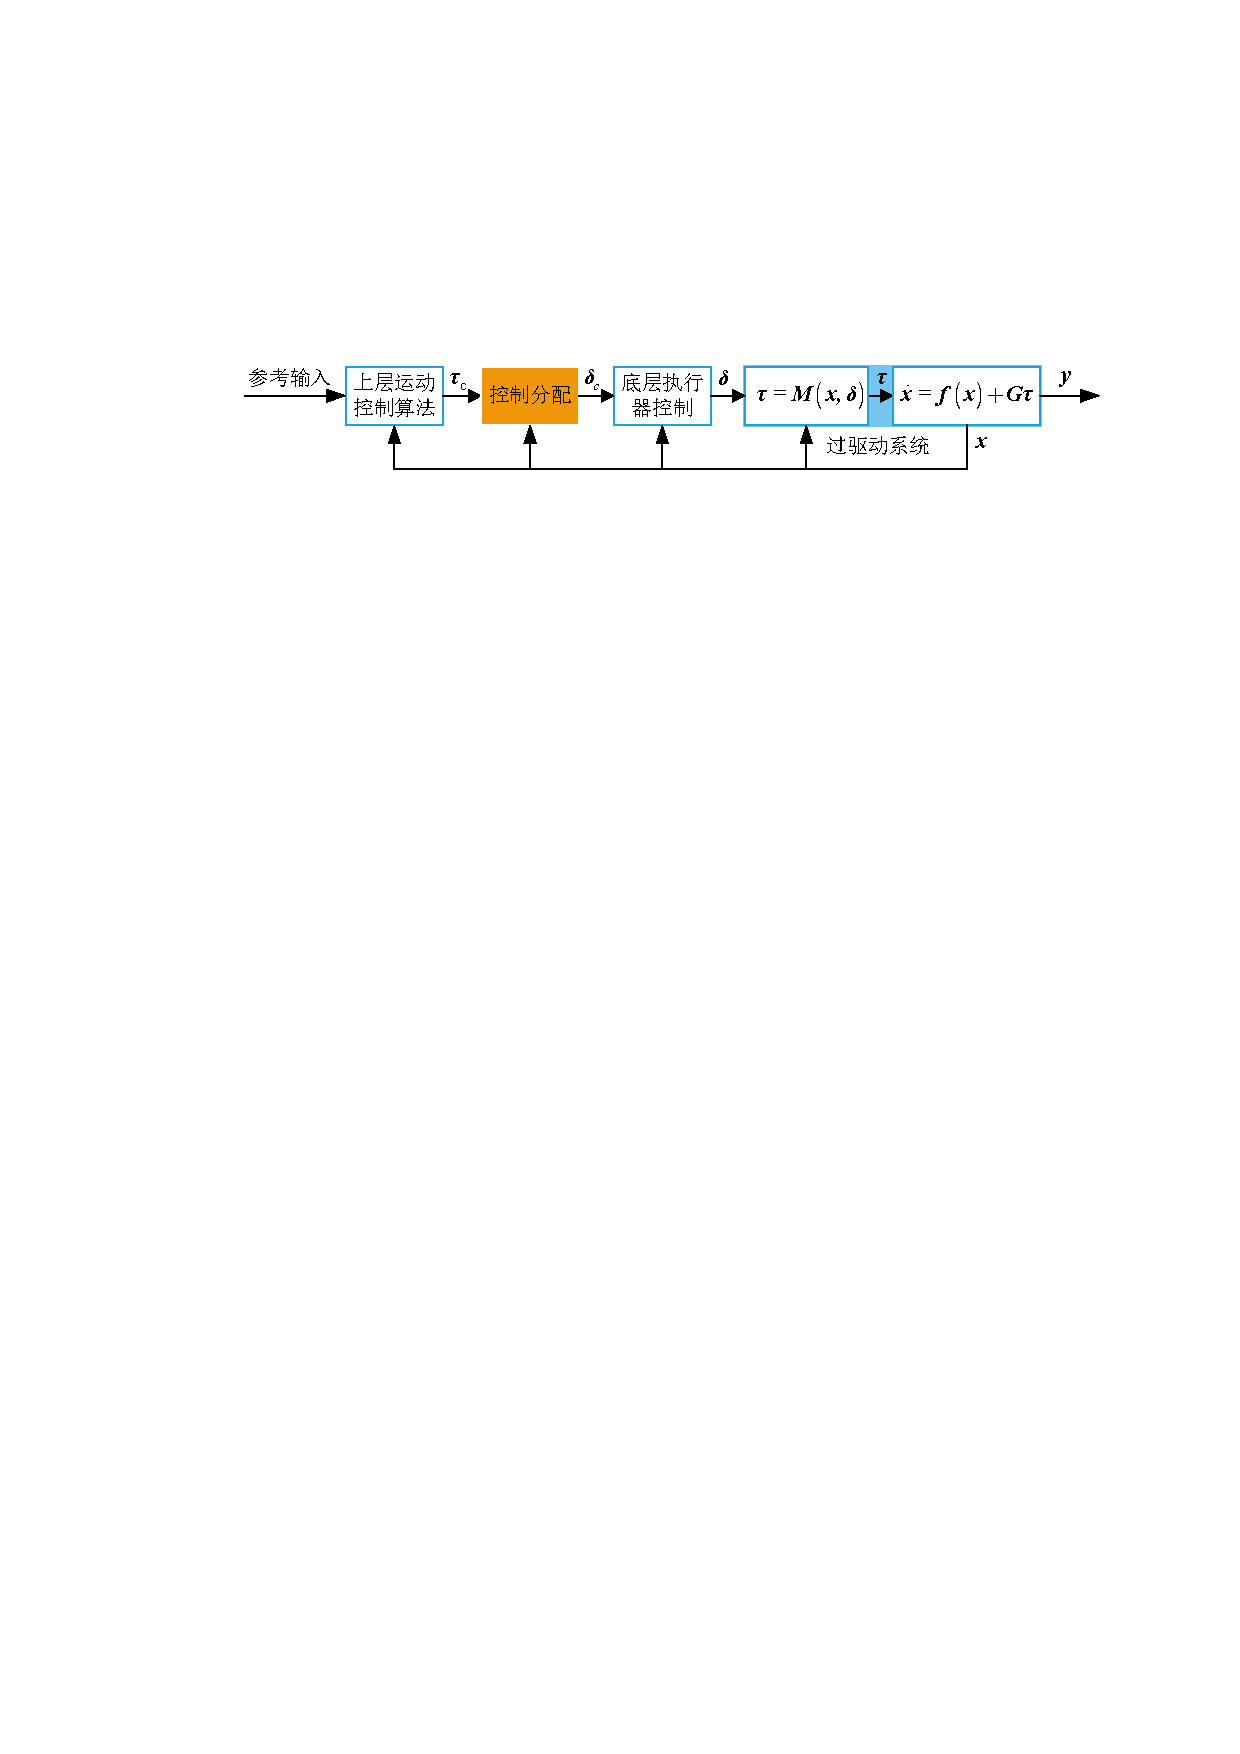
\includegraphics[scale=1]{Fig/Fig1.pdf}%
	\caption{\label{fig_system}基于控制分配的控制系统}
\end{figure}

容许控制集$\bm{\Omega}$通常是$\mathbb{R}^p$空间中的凸集。记
\begin{align}
\underline{\bm{\delta}}=\begin{bmatrix}
\delta_{1, \min } \\
\delta_{2, \min } \\
\vdots \\
\delta_{p, \min }
\end{bmatrix}, \quad \overline{\bm{\delta}}=\begin{bmatrix}
\delta_{1, \max } \\
\delta_{2, \max } \\
\vdots \\
\delta_{p, \max }
\end{bmatrix}, \quad \bm{\delta}=\begin{bmatrix}
\delta_{1} \\
\delta_{2} \\
\vdots \\
\delta_{p}
\end{bmatrix}
\end{align}
其中对$\forall i = 1, 2, \ldots, p$,若$\delta_{i,min} \leq {\delta }_i \leq {\delta}_{i,max}$,记为$\underline{\bm{\delta}} \leq \bm{\delta} \leq \overline{\bm{\delta}}$,则容许控制集为
\begin{align}
\bm{\Omega}=\left\lbrace   \bm{\delta} | \underline{\bm{\delta}} \leq \bm{\delta} \leq \bar{\bm{\delta}}\right\rbrace   \label{eq_effetor_limit}
\end{align}
式\eqref{eq_linear_model}所示操纵面的静态线性模型的重要性在于,可以在一个全局的范围观察一个系统的AMS,AMS是系统的属性,和控制分配算法无关。在具体实现中,在系统的每一个控制周期,控制分配采用的是式\eqref{eq_linear_model},除幅值约束外,还要考虑操纵面的速率约束。容许控制集变为幅值约束和速率约束的交集,相当于在每一个控制周期都有一个局部的幅值约束\cite{Durham_2017}。若记上一控制周期的控制输入为$\bm{\delta}_0$,控制周期为$T$,操纵面最大执行速率为$\bm{u}_m$,有局部约束
\begin{align}
-T\bm{u}_m \leq \bm{\delta}-\bm{\delta}_0 \leq T\bm{u}_m 
\end{align}
考虑式(13),取交集
\begin{align}
\overline{\bm{\delta}}^{\prime}=\min \left\lbrace \overline{\bm{\delta}}-\bm{\delta}_0, T\bm{u}_m\right\rbrace  \\
\underline{\bm{\delta}}^{\prime}=\max \left\lbrace \underline{\bm{\delta}}-\bm{\delta}_0,-T\ \right\rbrace
\end{align}
记$\Delta\bm{\delta}  = \bm{\delta}-{\bm{\delta}}_0$,则在每一控制周期进行控制分配时,容许控制集为
\begin{align}
\bm{\Omega}=\left\lbrace  \bm{\delta} | \underline{\bm{\delta}} \leq \bm{\delta} \leq \overline{\bm{\delta}}\right\rbrace \label{eq_effetor_limit_v}
\end{align}
结合式\eqref{eq_linear_model},控制分配问题和仅存在幅值约束的情形类似,区别是前者分配的起点是上一控制周期的控制输入 ,而后者分配的起点是$\bm{\delta}_0$空间的原点。考虑速率约束是系统的具体实现问题,仅考虑幅值约束得到的结论可应用到考虑速率约束的情形,因此在本文的讨论中不提及操纵面的速率约束,而在具体实现中默认考虑了速率约束。

应当指出,本文求解控制分配问题时,是在如下假设下进行:
\begin{enumerate}
	\item 假设已经获得系统的控制律,并且在控制律下子系统稳定。
	\item 假设执行器动态响应时间远远小于被控过程。
	\item 假设各个状态下的控制效率矩阵$\bm{B}$行满秩即$rank(\bm{B})=m$。
\end{enumerate}
%为简单起见,本文讨论涵道风扇式无人机的控制分配问题时,是在如下假设下进行:
%\begin{enumerate}
%	\item 假设已经获得系统的控制律,并且在控制律\eqref{eq_attitude_cpntrol_law}下姿态子系统\eqref{eq_attitude_sys}稳定。
%	\item 假设执行器动态响应时间远远小于被控对象。该无人机所用的力矩舵机带宽远大于被控对象,因此假设是合理的。
%	\item 假设各个状态下的控制效率矩阵$\bm{B}$已经通过仿真或试验数据获得。控制向量和力/力矩曲线$\bm{M}(\bm{x}, \bm{\delta})$亦即$ \bm{M}_{c} $随操纵面偏转角变化的曲线以离散数据的形式保存在计算机中,系统运行时将通过查表,利用插值法获取$\bm{B}$矩阵的元素。
%\end{enumerate}
%
\subsection{控制分配常用算法}
%
在控制分配问题中,式\eqref{eq_linear_model}可能无解,若有解则可能解不唯一。因此考虑将控制分配问题化为约束最优化问题求解,引入最优化指标。通常,代价函数的选择以尽量减少能量消耗或使执行器/执行器的磨损最小化等为标准。将控制分配问题归结为一个带约束的最优化问题,其形式通常为\cite{Johansen_2013}
\begin{alignat}{2}
\begin{split}
\mathop {{\text{minimize}}}\limits_{\bm{\delta},\bm{s}}\quad&{\|\bm{Q} s\|+J(\bm{x},\bm{\delta})} \\
\mbox{subject to}\quad
&\bm{\tau} -\bm{M}(\bm{x}, \bm{\delta})=\bm{s} \\
&\bm{\delta} \in \bm{\Omega }
\end{split} \label{eq_allo}
\end{alignat}
其中$ J(\bm{x},\delta) $为代价函数,$ s $为松弛变量。控制分配中常见的代价函数为
\begin{align}
J(\bm{x},\bm{\delta}) & =\frac{1}{2}\left(\bm{\delta}-\bm{\delta}_{p}\right)^{T} \bm{W}\left(\bm{\delta}-\bm{\delta}_{p}\right) \\
J(\bm{x},\bm{\delta}) & =\|\bm{W} \bm{\delta}\|
\end{align}
其中$\bm{W} \in \mathbb{R}^{p \times p}$为正定的加权矩阵,$ \bm{\delta}_{p} $是控制输入的首选值。为了反映分配误差最小化(松弛变量)作为首要优化目标,而代价函数作为次要优化目标,$ \bm{W} $通常选远小于
$ \bm{Q} $。

本节介绍几种常用于飞行器控制中的控制分配算法。
\subsubsection{伪逆法}
%
若不考虑任何操纵面约束,则对给定$ \bm{\tau} $,线性方程组$ \bm{\tau}=\bm{B}\bm{\delta} $总是有解,控制分配问题可描述为
\begin{alignat}{2}
\begin{split}
\mathop {{\text{minimize}}}\limits_{\bm{\delta}}\quad&{\frac{1}{2}\left\|\bm{W}\left(\bm{\delta}-\bm{\delta}_{p}\right)\right\|^{2} } \\
\mbox{subject to}\quad
&\bm{\tau}=\bm{B} \bm{\delta} 
\end{split} \label{inv}
\end{alignat}
注意到$ \bm{B} $是行满秩矩阵,因此问题有闭解\cite{Boyd_2004a}
\begin{align}\bm{\delta}=(\bm{I}-\bm{C B}) \bm{\delta}_{p}+\bm{C \tau}\end{align}
其中$\bm{C}=\bm{W}^{-1} \bm{B}^\top \left(\bm{B} \bm{W}^{-1} \bm{B}^\top \right)^{-1}$。若取加权矩阵为单位阵$ \bm{W}=\bm{I} $,对给定$\bm{\tau }$,解为$ \bm{\delta}=\bm{B}^+ \bm{\tau} $
,其中$\bm{B}^+$为$\bm{B}$的伪逆(pseudo-inverse),即$ \bm{B}^+= \bm{B}^\top (\bm{B} \bm{B}^\top)^{-1} $。这种控制分配称为伪逆法。

\subsubsection{加权最小二乘法}
考虑执行器受限的控制分配可以描述为\cite{Harkegard_2002}:根据伪控制输入$ \bm{\tau} $计算舵机偏角$\bm{\delta } \in \bm{\Omega} $,如果$ \bm{\tau}=\bm{B}\bm{\delta} $有解,则选一个最佳的解。如果由于执行器幅值和速度约束,$ \bm{\Omega} $中无法找到满足等式$ \bm{\tau}=\bm{B}\bm{\delta} $的解,则希望降低一点性能并最小化分配误差\cite{Harkegard_2002},即$ \bm{\tau}-\bm{B}\bm{\delta} $尽可能小。此时控制分配问题可以归结为一个含不等式约束的加权最小二乘(WLS)问题:
\begin{alignat}{2}
\begin{split}
\mathop {{\text{minimize}}}\limits_{\bm{\delta}}\quad&{\frac{1}{2}\left\|\bm{W}_{\delta}\left(\bm{\delta}-\bm{\delta}_{p}\right)\right\|^{2}+\frac{1}{2} \gamma^{2}\left\|\bm{W}_{\tau}\left(\bm{\tau}-\bm{B} \bm{\delta}\right)\right\|^{2} } \\
\mbox{subject to}\quad
&\underline{\bm{\delta}} \leq \bm{\delta} \leq \overline{\bm{\delta}}
\end{split} \label{wls}
\end{alignat}
其中$ \left\|r \right\|^{2}=r^\top r $,即定义为向量$ r $的2-范数。$ \bm{\delta}_{p} $是首选的舵面偏角,一般为零向量,希望舵机尽量小的偏转。$ \bm{W}_{\delta} $、$ \bm{W}_{\tau} $是相应的加权矩阵。$ \gamma $是取值为正实数的权值因子,为了强调优化的首要目的是尽可能减小分配误差,因此γ一般取较大的值。

通常求解式\eqref{wls}是将其化为二次规划问题的标准形式\cite{Nocedal_2006}
\begin{alignat}{2}
\begin{split}
\mathop {{\text{minimize}}}\limits_{\bm{\delta}}\quad&{  \frac{1}{2}\|\bm{A} \bm{\delta}-\bm{b}\|^{2}   } \\
\mbox{subject to}\quad
&  \bm{C}\bm{\delta} \geq \bm{U}
\end{split} 
\end{alignat}
其中
\begin{align*}
\bm{A}=\left[ \begin{array}{c}
\gamma \bm{W}_{\tau} \bm{B} \\
\bm{W}_{\delta}
\end{array}\right] , \quad 
\bm{b}=\left[ \begin{array}{c}
\gamma \bm{W}_{\tau} \bm{\tau} \\
\bm{W}_{\delta} \bm{\delta}_{p}
\end{array}\right] , \quad 
\bm{C}=\left[ \begin{array}{c}
\bm{I} \\
-\bm{I}
\end{array}\right] ,\quad
\quad \bm{U}=\left[ \begin{array}{c}
\underline{\bm{\delta}} \\
-\overline{\bm{\delta}}
\end{array}\right]
\end{align*}
然后用有效集方法求解\cite{Smeur_2017,Harkegard_2002}。
\subsubsection{直接分配法}
%
为了对任意给定$\bm{\tau} \in \bm{\Phi}$,都返回一个容许控制,设$\bm{\tau}_{max} $是AMS中矢量$\bm{\tau} $方向上幅值最大的矢量,定义比例因子$\alpha=\left\|\bm{\tau}_{\max }\right\|^{2} /\left\|\bm{\tau}\right\|^{2}$。控制分配问题表述为求解一组$\alpha$、$ \bm{\delta} $满足$\alpha\bm{\tau}=\bm{B}\bm{\delta}$且 $\bm{\delta } \in \bm{\Omega}  $。用最优化问题的形式来表达,可表示为\cite{Bodson_2002}
\begin{alignat}{2}
\begin{split}
\mathop {{\text{minimize}}}\limits_{\bm{\delta},\alpha}\quad&{-\alpha} \\
\mbox{subject to}\quad
&\alpha\bm{\tau}=\bm{B}\bm{\delta} \\
&\underline{\bm{\delta}} \leq \bm{\delta} \leq \overline{\bm{\delta}} \\
&0 \leq \alpha \leq 1
\end{split} \label{dir}
\end{alignat}
求解式\eqref{dir}即为直接分配法。具体算法实现中, $ \alpha $的取值可以放宽为大于等于零的实数,若 $ \alpha >1 $,则将解$ \bm{\delta} $缩小$ \alpha $倍。可将式\eqref{dir}化为线性规划问题的标准形式,用单纯形法求解该最优化问题\cite{Bodson_2002}。该方法可对任意可达的 $ \bm{\tau} $无误差分配,即返回一个容许控制,使$ \bm{\tau}=\bm{B}\bm{\delta} $ 。对不可达的 $ \bm{\tau} $ ,仅能满足 $ \alpha\bm{\tau}=\bm{B}\bm{\delta} $,$ 0 \leq \alpha \leq 1 $ ,分配误差为 $ \bm{\tau}-\bm{B}\bm{\delta} $。比例因子的作用是减小 $ \bm{\tau} $ 的幅值,因此该方法具有方向保持的特性,是一种几何算法。在文献\parencite{Durham_2017}中,直接分配法被用来求AMS,在航空航天应用中,AMS是三维空间中的凸多面体。
\subsection{控制分配算法的可达集}
分配算法的优劣可以从多方面进行评价,如算法时间复杂度\cite{Harkegard_2002},可达集大小\cite{Durham_2017}等。利用可达集的大小来评价分配算法较直观,在本文中会多次使用,因此本节引入所需的一些符号。

用$\partial(\cdot)$ 表示包围某点集的凸包,包围容许控制集、AMS的凸包分别记为 $\partial(\bm{\Omega})$、 $\partial(\bm{\Phi})$。对所有可达的  $ \bm{\tau} $,某一分配算法返回的所有的容许控制的集合记为$\bm{\Theta} $ 。记$\bm{\Pi} $ 为 $\bm{\Theta} $通过控制效率矩阵$ \bm{B} $ 从$ {{\mathbb{R}}^p} $ 空间映射到$ {{\mathbb{R}}^m} $ 空间得到的集合,称为某分配算法的可达集。对$ m=3 $ 的情形,使用$\bm{\Pi} $ 和$ \bm{\Phi} $ 的体积之比的百分数表示某分配算法的品质因数 ,可作为衡量算法优劣的指标\cite{Durham_2017}。


%\begin{align}\left\{\begin{array}{l}
%\dot{x}_{1}^{*}(t)=x_{2}^{*}(t) \\
%\dot{x}_{2}^{*}(t)=\Phi\left(x_{1}^{*}(t), x_{2}^{*}(t)\right), \Phi(0,0)=0
%\end{array}\right.	\label{eq_sec_ref_sys}
%\end{align}


%将$\bm{g}\left( \bm{x}, \bm{\delta} \right)$做矩阵分解
%\begin{align}
%\bm{g}\left( \bm{x}, \bm{\delta} \right)=\bm{G}\bm{M}(\bm{x}, \bm{\delta}) 
%\end{align}
%引入伪控制输入


%将式\eqref{eq_sys}化为
%\begin{align}
%\left\{\begin{array}{l}
%\dot{\bm{x}} =\bm{f}(\bm{x})+\bm{G} \bm{\tau} \\
%\bm{\dot{\delta} } = \bm{k}\left( \bm{\delta},\bm{\zeta} \right)  \\
%\bm{y} =\bm{h}(\bm{x} ) 
%\end{array}\right.\label{eq_intro_v_sys}
%\end{align}

%考虑执行器受限的控制分配可以描述为\cite{Harkegard_2002}:根据伪控制指令$ \bm{\tau} $计算舵机偏角$\bm{\delta } \in \bm{\Omega} $,如果$ \bm{\tau}=\bm{B}\bm{\delta} $有解,则选一个最佳的解。如果由于执行器幅值和速度约束,$ \bm{\Omega} $中无法找到满足等式$ \bm{\tau}=\bm{B}\bm{\delta} $的解,则希望降低一点性能并最小化分配误差,即$ \bm{\tau}-\bm{B}\bm{\delta} $尽可能小。此时控制分配问题可以归结为一个含不等式约束的二次规划问题。文献\parencite{Harkegard_2002}利用有效集方法(Active Set Method)求解该二次规划问题,并指出该解法降低了时间复杂度。虽然该方法已经在很多系统中得到应用,例如,文献\parencite{Smeur_2017}利用该方法解决四旋翼无人机的控制分配问题,但正如前文所述的涵道飞行器的诸多独特性,在下一节我们将考虑从另一个角度解决涵道无人机的控制分配问题。
%\parencite{Pflimlin_2007a,Zhao_2015,Peddle_2009}

\section{单涵道控制分配}
\subsection{操纵面模型}
定义单涵道无人机的操纵面偏转角矢量$\bm{\delta } = [\delta_1 \quad \delta_2 \quad \delta_3 \quad \delta_4]^\top$,如第二章所述,将其称为控制向量。将式\eqref{eq_M_c}改写为
\begin{align}
\bm{M}_{c}=\begin{bmatrix} \tau_{x} \\ \tau_{y} \\ \tau_{z} \end{bmatrix}=\begin{bmatrix}
-l_{1} & 0 & l_{1} & 0 \\
0 & -l_{1} & 0 & l_{1} \\
l_{2} & l_{2} & l_{2} & l_{2}
\end{bmatrix} k_{\delta} (V_i+V_c)^2 \bm{\delta}
\end{align}
取驱动力矩为伪控制输入,即$\bm{\tau } =\bm{M}_{c}$,结合式\eqref{eq_linear_model},得控制效率矩阵为
\begin{align}
\bm{B}=k_{\delta}(V_i+V_c)^2\begin{bmatrix}
-l_{1} & 0 & l_{1} & 0 \\
0 & -l_{1} & 0 & l_{1} \\
l_{2} & l_{2} & l_{2} & l_{2}
\end{bmatrix}
\label{eq_B}
\end{align}	
上式隐含$\bm{B}$和系统状态相关,易知被控量的自由度小于控制量的维数,因此姿态子系统是一个过驱动系统,其控制分配问题可基于式\eqref{eq_linear_model}、式\eqref{eq_B}并结合操纵面约束进行。


%本章第一节先介绍常用的两种控制分配方法:伪逆法和直接分配法,将其应用到涵道风扇式飞行器的控制分配问题中,并对比了两种分配方法的可达集。在第二节中,针对两种常用方法的不足,提出一种优先级分配方法。
%

基于第三章设计的自抗扰控制律,考虑控制分配问题之后,单涵道无人机的姿态控制系统框图如图\ref{tradi_base_ADRC}所示。其中$ \bm{v}_1=[v_{r1} \quad v_{p1}\quad v_{y1} ]^\top$,$ \bm{v}_2=[v_{r2} \quad v_{p2}\quad v_{y2} ]^\top $,$ \hat{\bm{x}}_1=[\hat{x}_{r1} \quad \hat{x}_{p1}\quad \hat{x}_{y1} ]^\top $,$ \hat{\bm{x}}_2=[\hat{x}_{r2} \quad \hat{x}_{p2}\quad \hat{x}_{y2} ]^\top $,$ \hat{\bm{x}}_3=[\hat{x}_{r3} \quad \hat{x}_{p3}\quad \hat{x}_{y3} ]^\top $,$ \bm{u}_0=[u_{r0} \quad u_{p0}\quad u_{y0} ]^\top $。$[\varphi_c \quad \theta_c \quad \psi_c]^\top$为欧拉角给定。在下一节将分析图\ref{tradi_base_ADRC}所示的系统应该常规控制分配方法的不足,进而引入优先级分配方法。
\begin{figure}[htbp]
	\centering	
	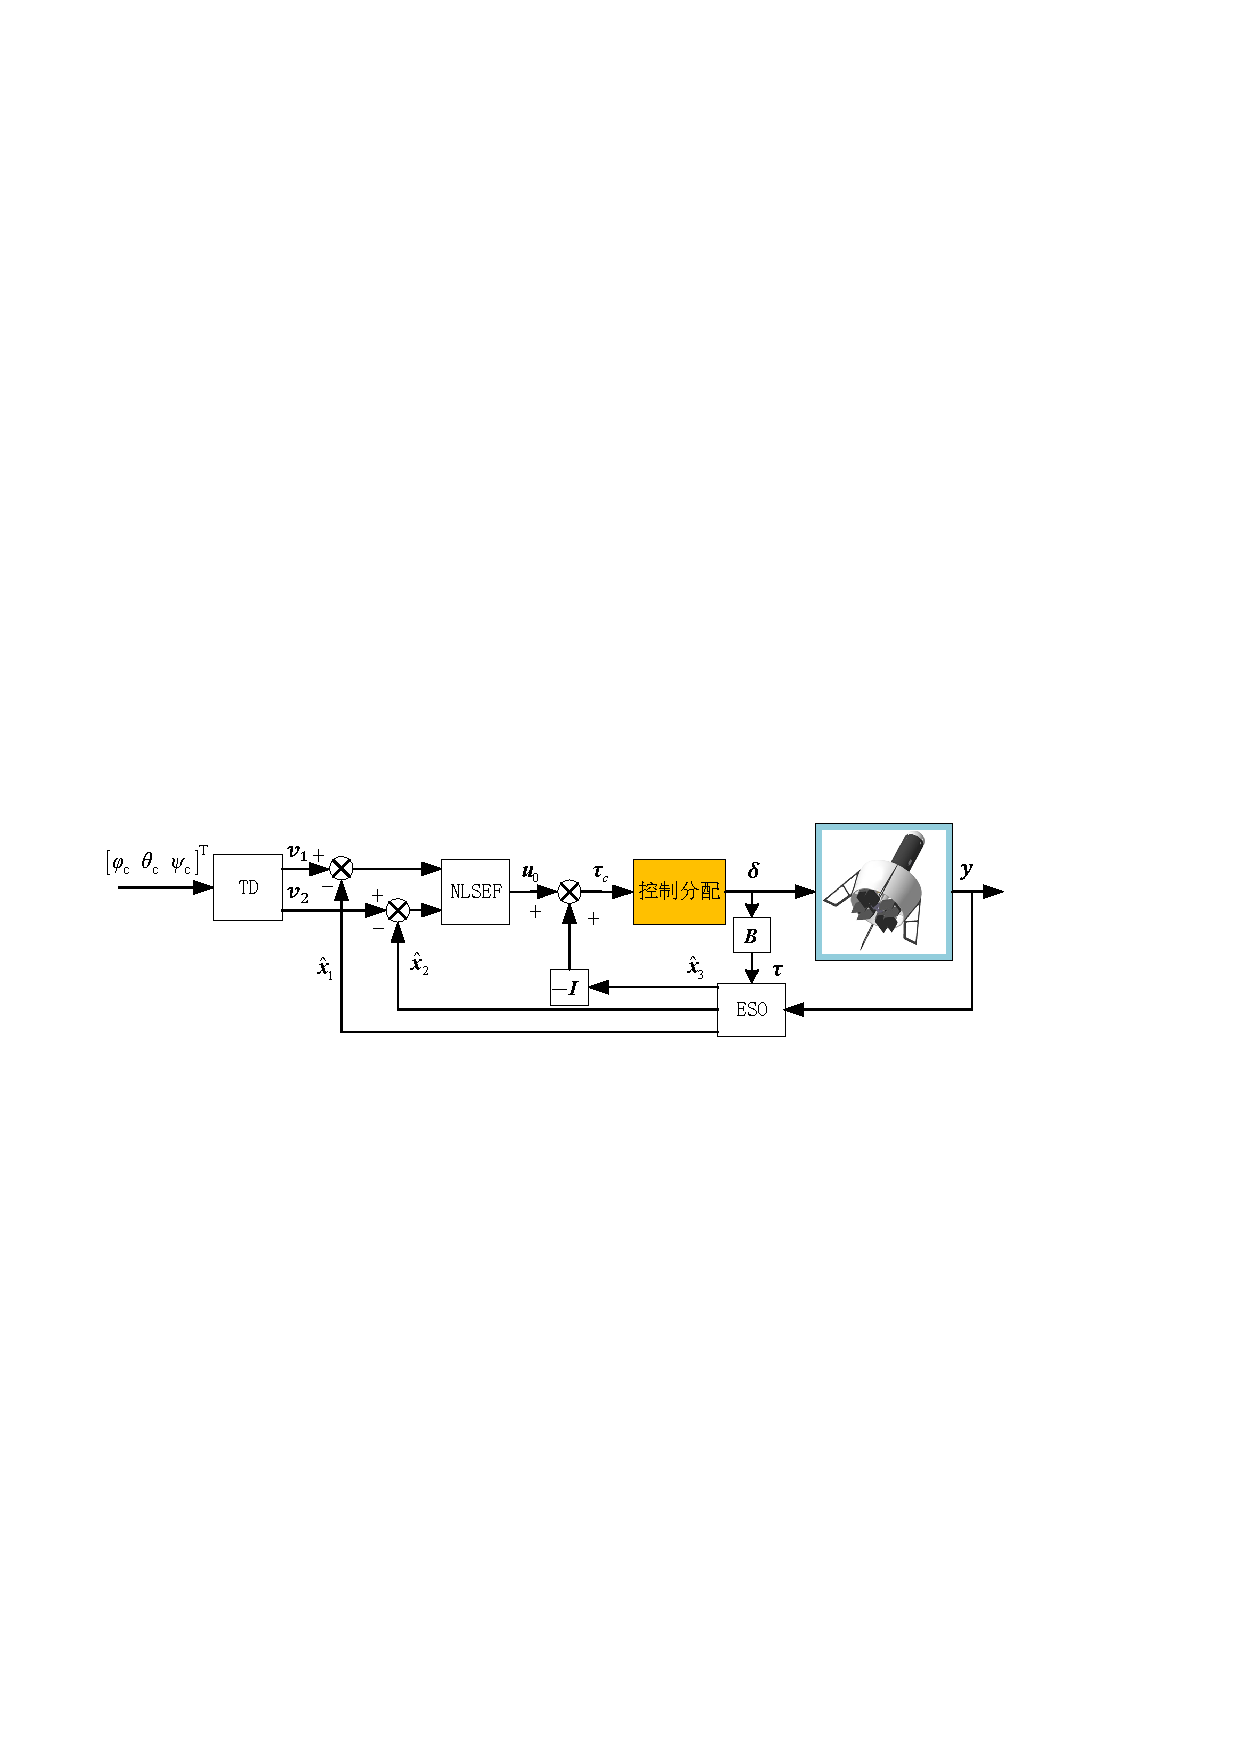
\includegraphics[scale=1]{Fig/tradi_base_ADRC.pdf}
	\caption{\label{tradi_base_ADRC}姿态控制系统框图}
\end{figure}
\subsection{常规方法的局限性}
目前,包括文献\parencite{Ahmadi_2011,Aruneshwaran_2013a,Binetti_2007,Chen_2019,Emami_2018,Fan_2018,Hassanalian_2017,Hess_2008,Johnson_2005,Lipera_2001,Manzoor_2020,Naldi_2010,Ohanian_2010,Ohanian_2012,Peddle_2009,Pflimlin_2006,Pflimlin_2007,Pflimlin_2007a,Sharifzadeh_2019,Sheng_2015,Straub_2016,Zhao_2008,Zhao_2015}在内的很多文献,在研究涵道风扇式无人机的控制问题时,都没有展开讨论控制分配问题,所用的分配方法实际上等价于伪逆法。由于操纵面约束的存在,对任意给定$\bm{\tau} \in \bm{\Phi} $,$ \bm{\delta} $可能不在容许控制集内,即$\bm{\delta } \notin \bm{\Omega} $,实际执行的控制输入是 经过限幅后的值。

试验测得在悬停状态下的 $ \bm{B} $矩阵为
\begin{align}\bm{B}=\left[\begin{array}{cccc}
-0.5393 & 0 & 0.5393 & 0 \\
0 & -0.5393 & 0 & 0.5393 \\
0.2099 & 0.2099 & 0.2099 & 0.2099
\end{array}\right]	\label{control_effectiveness_matrix}
\end{align}
其操纵面约束为
\begin{align}\underline{\bm{\delta}}=\left[\begin{array}{l}
-20^{\circ} \\
-20^{\circ} \\
-20^{\circ} \\
-20^{\circ}
\end{array}\right], \overline{\bm{\delta}}=\left[\begin{array}{c}
20^{\circ} \\
20^{\circ} \\
20^{\circ} \\
20^{\circ}
\end{array}\right]	\label{position_constraints}
\end{align}

利用MATLAB$^\circledR$分别绘制出伪逆法和直接分配法的可达集 $\bm{\Pi}_1 $ 、$\bm{\Pi}_2 $  ,如图\ref{fig_AMS}所示。由算法流程易知直接分配法的可达集$\bm{\Pi}_2=\bm{\Phi} $ ,分别计算  $\bm{\Pi}_1 $ 、$\bm{\Pi}_2 $ 的品质因数为 ${\gamma _1} = 71.99\% $、${\gamma _2} = 100\% $。对 $ \bm{\Phi}$中的所有力矩,任何无法返回容许控制的控制分配方法都没有充分利用飞机的控制性能\cite{Durham_2017},因此在涵道风扇式无人机的控制分配中广泛应用的伪逆法,实际上牺牲了部分控制能力。
\begin{figure}[htbp]
	\centering	
	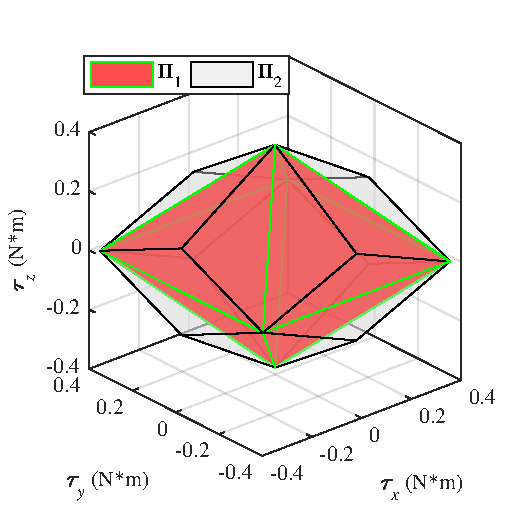
\includegraphics[scale=1]{Fig/Fig4.pdf}
	\caption{\label{fig_AMS}伪逆法和直接分配法的可达集对比}
\end{figure}

直接分配法对不可达的 $ \bm{\tau} $ ,将被保方向地限制在$\partial(\bm{\Phi})$ 上,其分配误差为$(1-\alpha)\bm{\tau}$,即每一个分量上都有分配误差。WLS法的品质因数和直接分配法相同,WLS法对不可达的 $ \bm{\tau} $,将取最接近AMS边界的一点进行分配,没有保方向特性。上述方法相对于伪逆法都有所改善,但由图\ref{fig_AMS}可知,单涵道的AMS太小,即使扩大算法的可达集到其极限值AMS,作用于系统的力矩仍会经常在$\partial(\bm{\Phi})$附近,执行器饱和的几率较大。对不可达的伪控制输入,总和产生分配误差。

然而,在某些情况下为了满足控制需求,控制律有些分量应尽可能无分配误差。例如第三章中的自抗扰控制律\eqref{eq_intro_v_sys},为确保系统正确运行,补偿总和扰动的分量$ -I z_{3}(k) $需要尽可能无误差分配。该分量将系统化为线性系统,是系统稳定的前提。
\subsection{优先级分配}
%
针对单涵道上使用常规解法的遇到的问题,我们提出优先级控制分配方法,先将期望力矩进行优先级分解,若 $ \bm{\tau} $不可达,将其与$\partial(\bm{\Phi})$ 的交点进一步优化,使得 $ \bm{\tau} $ 的高优先级分量尽可能无误差分配,仅低优先级分量产生分配误差。
%
\subsubsection{控制律的优先级分解}
%
期望力矩$ \bm{\tau} $由式\eqref{eq_intro_v_sys}所示系统的控制律$ \bm{\tau}_c $和截距项确定 ,$ \bm{\tau} \in {\mathbb{R}}^p$可以在$ {\mathbb{R}}^m $ 空间按坐标轴或不同控制效果做矢量分解,分解后按控制目标划分优先级。

以滚转通道为例,对自抗扰控制律进行分解,将控制律\eqref{eq_roll_cl}分解为
\begin{align}
\tau_{xc}=\tau _{x1}+\tau_{x2}
\end{align}
其中$ \tau_{x 1}  \triangleq-I z_{3}(k) $,$ \tau_{x 2}  \triangleq u_{r0}  $。同理,对俯仰、偏航通道的控制律$\tau_{yc}$、$\tau_{zc}$做类似的分解,总的控制律可分解为
\begin{align}
\bm{\tau_{\mathrm{c}}}=\bm{\tau_{1}}+\bm{\tau_{2}}	\label{control_law}
\end{align}
\begin{equation}
\bm{\tau}_c \triangleq  \begin{bmatrix}
\tau_{x c} \\
\tau_{y c} \\
\tau_{z c}
\end{bmatrix}, 
\bm{\tau}_{1} \triangleq  \begin{bmatrix}
\tau_{x 1} \\
\tau_{y 1} \\
\tau_{z 1}
\end{bmatrix},
\bm{\tau}_{2} \triangleq  \begin{bmatrix}
\tau_{x 2} \\
\tau_{y 2} \\
\tau_{z 2}
\end{bmatrix}
\end{equation}
其中$\bm{\tau}_1$包含对系统总和扰动的补偿。$\bm{\tau}_2$通常是应用状态反馈设计的,因此和系统动态响应相关。在该控制律下,系统能按照预期运行的首要前提是$\bm{\tau}_1$可以抵消系统总和扰动,将非线性系统化为线性系统,而后才可以设计误差反馈$\bm{\tau}_2$,使系统稳定(或跟踪输入)。因此将控制律分解后,可以认为$\bm{\tau}_1$分量优先级较高,而$\bm{\tau}_2$分量优先级较低。


应当指出,这些分解是人为规定的,还可以根据不同需求做其他分解。基于反馈线性化方法设计的控制律中,都可以做和上述方法类似的分解,因为其本质都是先将非线性系统化为线性系统,再对该线性系统设计误差反馈律,例如非线性动态逆(NDI)及增量非线性动态逆\cite{Wang_2019}(INDI),其思路和ADRC是相似的。文献\parencite{Smeur_2017,Buffington_1997}讨论了NDI控制律的分解,以及文献\parencite{Yu_2015}讨论了串级PID控制律的分解。
%
\subsubsection{优先级控制分配}
%
在控制分配环节控制律作为期望力矩,假设期望力矩已经分解为$\bm{\tau}=\bm{\tau}_1+\bm{\tau}_2+\ldots+\bm{\tau}_k$,其中从$\bm{\tau}_1$到$\bm{\tau}_k$优先级依次降低。为保证高优先级分量不产生分配误差,考虑仅对优先级最低的$\bm{\tau}_k$进行缩放,引入比例因子$\alpha$,求解下式
\begin{alignat}{2}
\begin{split}
\mathop {{\text{minimize}}}\limits_{\bm{\delta},\alpha}\quad&{-\alpha} \\
\mbox{subject to}\quad
&\bm{B}\bm{\delta}=\bm{\tau}_1+\bm{\tau}_2+\ldots+\alpha\bm{\tau}_k \\
&\underline{\bm{\delta}} \leq \bm{\delta} \leq \overline{\bm{\delta}} \\
&0 \leq \alpha \leq 1
\end{split} \label{eq_prio1}
\end{alignat}	
上式的解可以分为两种情况:
\begin{enumerate}
	\item 若式\eqref{eq_prio1}有解,则控制分配结束,返回该最优解$\bm{\delta}$。此时若$\alpha=1$,表示$\bm{\tau}$可达,求解式(33)等价于对$\bm{\tau}$用直接分配法求解容许控制。若 ,表示$\bm{\tau}$不可达但$\bm{\tau}_1+\bm{\tau}_2+\ldots+\alpha \bm{\tau}_k $在$\partial(\bm{\Phi})$ 上,仅改变$\bm{\tau}_k$的幅值即可返回容许控制,因此仅在$\bm{\tau}_k$方向有分配误差。
	\item 若式\eqref{eq_prio1}无解,则在$\bm{\tau}$中把低优先级分量$\bm{\tau}_k$去掉,此时期望力矩变为$\bm{\tau '}=\bm{\tau}_1+\bm{\tau}_2+\ldots+\bm{\tau}_{k-1}$,此种情况表明$\bm{\tau '}$不可达。同理,仅对优先级最低的 进行缩放,求解下式
	\begin{alignat}{2}
	\begin{split}
	\mathop {{\text{minimize}}}\limits_{\bm{\delta},\alpha}\quad&{\alpha} \\
	\mbox{subject to}\quad
	&\bm{B}\bm{\delta}=\bm{\tau}_1+\bm{\tau}_2+\ldots+\alpha\bm{\tau}_{k-1} \\
	&\underline{\bm{\delta}} \leq \bm{\delta} \leq \overline{\bm{\delta}} \\
	&0 \leq \alpha \leq 1
	\end{split} \label{eq_prio2}
	\end{alignat}	
	若\eqref{eq_prio2}有解则分配结束,若无解,则去掉$\bm{\tau}_{k-1}$重复上述过程。注意到,若重复了$k-1$次该过程之后仍然无解,说明$\bm{\tau}_{1}$不可达,第 次求解时等价于对$\bm{\tau}_{1}$用直接分配法求解控制向量。因此该问题在有限次循环后一定有解。
\end{enumerate}	

上述求解过程可以表示为从$s=k$开始求解下式	
\begin{alignat}{2}
\begin{split}
\mathop {{\text{minimize}}}\limits_{\bm{\delta},\alpha_s}\quad&{-\alpha_s} \\
\mbox{subject to}\quad
&\bm{B}\bm{\delta}=\bm{\tau}_1+\bm{\tau}_2+\ldots+\alpha\bm{\tau}_{k} \\
&\underline{\bm{\delta}} \leq \bm{\delta} \leq \overline{\bm{\delta}} \\
&0 \leq \alpha_s \leq 1   \\
&\alpha_j={\begin{cases}
	0 &  j<s,\\
	1 &  j>s.
	\end{cases}\quad j=1,2, \ldots, k.}
\end{split} \label{eq_prio}
\end{alignat}
其中$s=k,k-1,\ldots ,1$,若无可行解,则令$s=s-1$,循环求解式\eqref{eq_prio}直到有可行解时停止,即为优先级分配方法。当$\bm{\tau}$可达时,求解式\eqref{eq_prio}等价于直接分配法;当$\bm{\tau}$不可达时,若在 次求解式\eqref{eq_prio}后返回最优解,则$\bm{\tau}_1,\bm{\tau}_2,\ldots,\bm{\tau}_k$都是无误差分配,其中$0\le i\le k$。当控制律中没有做优先级分解时,等价于$\bm{\tau}=\bm{\tau}_1$,优先级分配法退化为直接分配法。从式\eqref{eq_prio}可知该方法的可达集和直接分配法一样,品质因数为$100\%$。
\begin{figure}[htbp]
	\centering	
	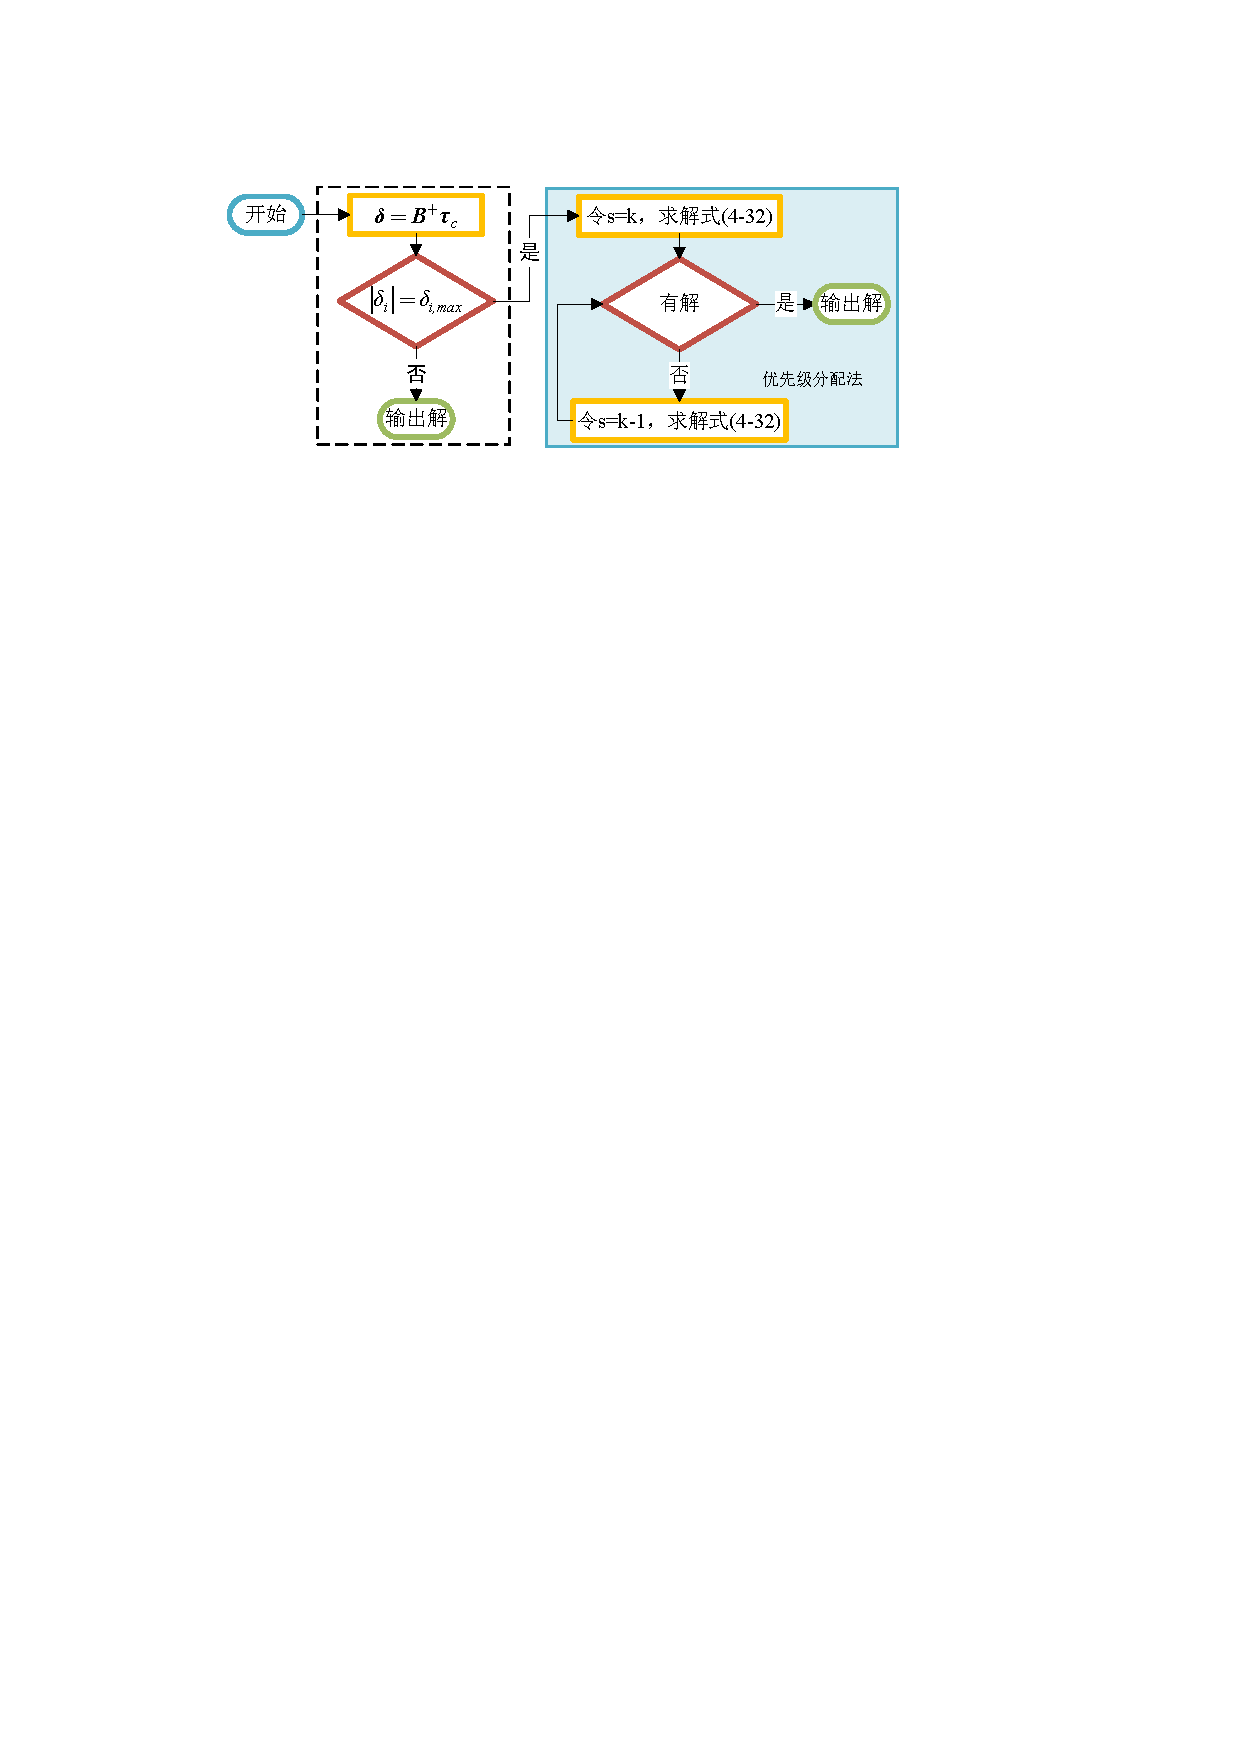
\includegraphics[scale=1]{Fig/Fig5.pdf}
	\caption{\label{fig_sequence}优先级分配法流程图}
\end{figure}
在具体实现中,为了减小计算量,求解式\eqref{eq_prio}前,可先用伪逆法计算一个参考值,若该参考值已经使操纵面饱和,再求解式\eqref{eq_prio},否则输出该参考值即可。应该指出,这一步参考值的计算不是必须的,但分配小幅值力矩时使用伪逆法,可以带来诸多好处,例如可以解决因考虑速率约束进行控制分配时带来的恢复问题\cite{Durham_2017}。控制分配流程图如图\ref{fig_sequence}所示,虚线方框内是可选的步骤,蓝色方框内是优先级分配方法流程。
\begin{figure}[htbp]
	\centering	
	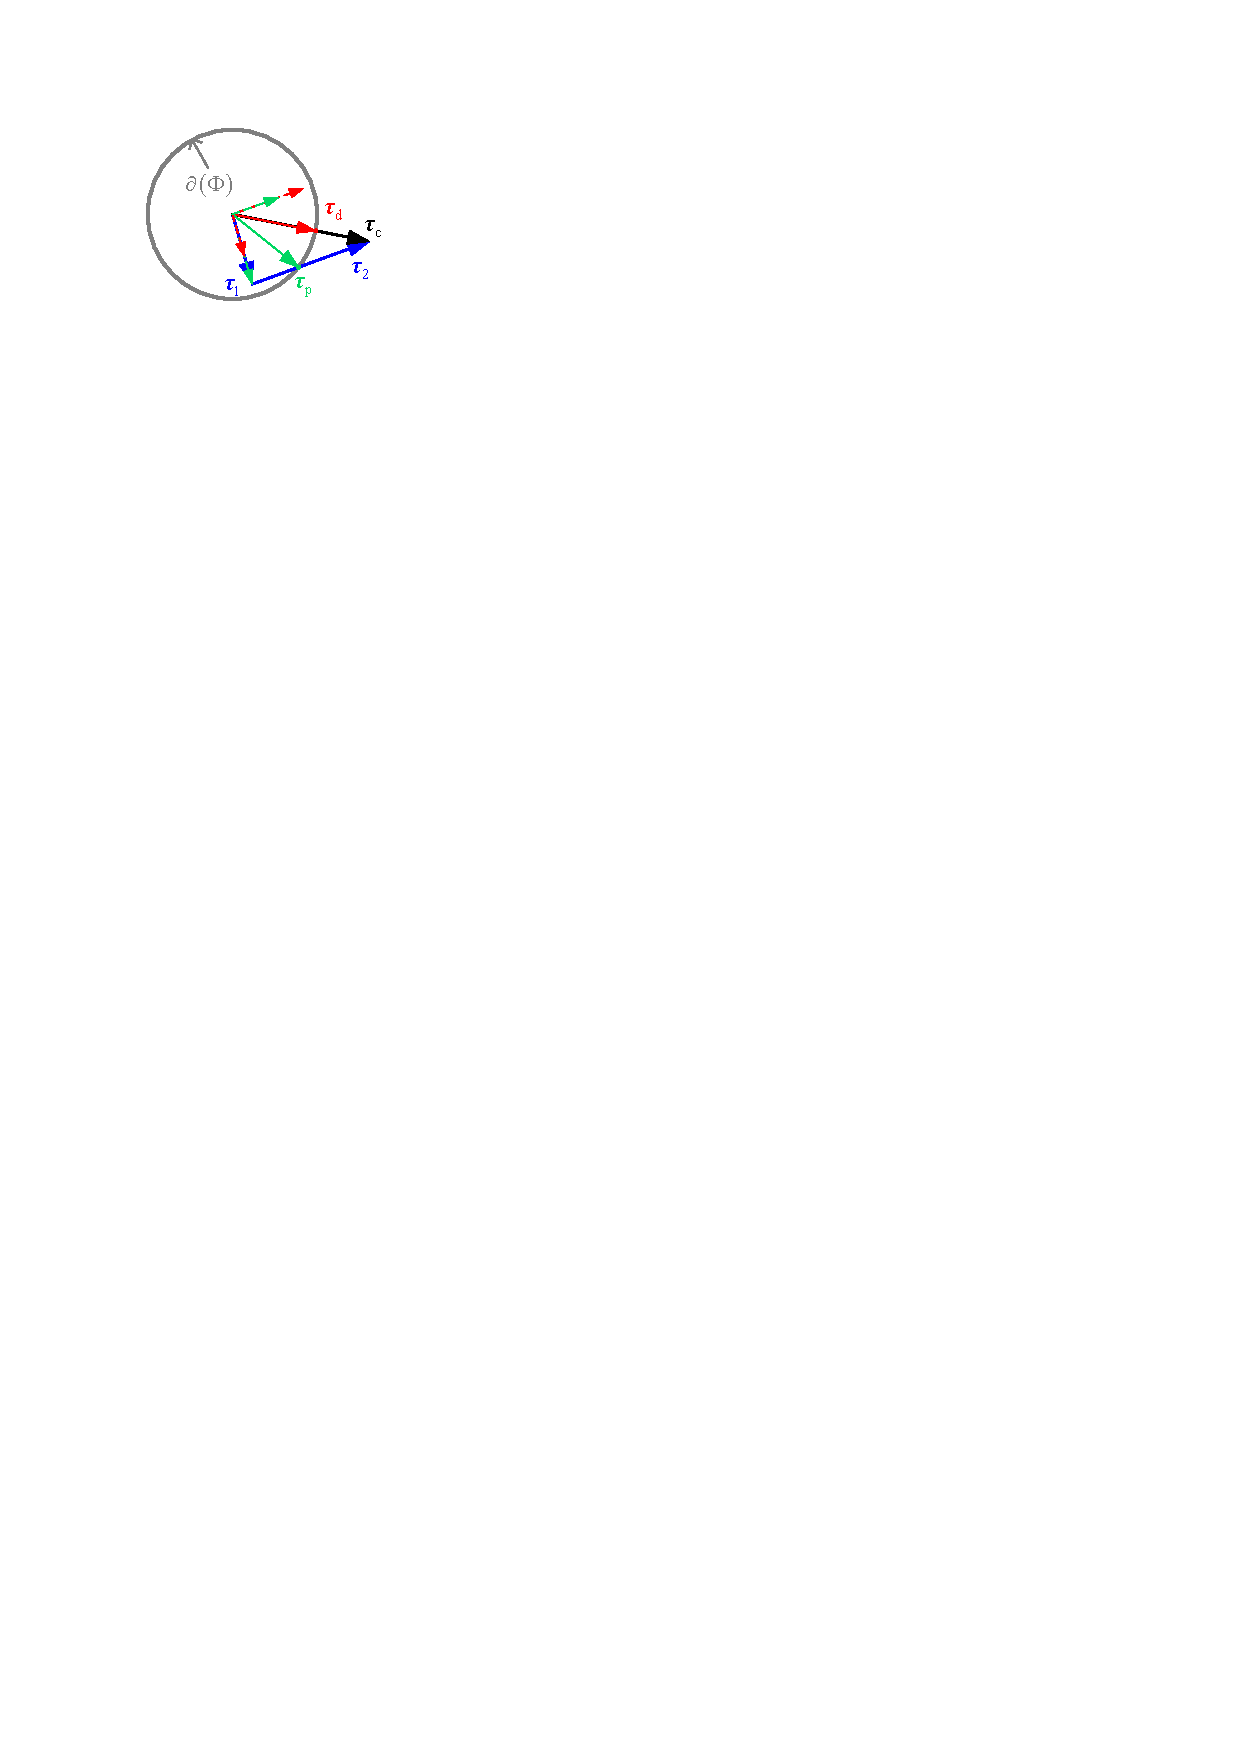
\includegraphics[scale=1]{Fig/Fig6.pdf}
	\caption{\label{fig_case}二维优先级分配法和直接分配法对比}
\end{figure}

图\ref{fig_case}给出一种2维力矩空间的例子,若$\bm{\tau}=\bm{\tau}_1+\bm{\tau}_2$,且$m=2$,$\bm{\tau}$不可达。分别用直接分配法、优先级分配法求解控制向量,再通过 映射到 空间得$\bm{\tau}_d$、$\bm{\tau}_p$。将$\bm{\tau}_d$、$\bm{\tau}_p$沿$\bm{\tau}_1$、$\bm{\tau}_2$方向做矢量分解,如图\ref{fig_case}所示。$\bm{\tau}_d$在每个分量方向上都有分配误差。$\bm{\tau}_p$则仅在低优先级分量$\bm{\tau}_2$方向上有分配误差,而在高优先级分量$ \bm{\tau}_1 $方向没有分配误差。

使用优先级控制分配后,图\ref{tradi_base_ADRC}所示的系统结构框图变为图\ref{prio_base_ADRC}所示。
\begin{figure}[htbp]
	\centering	
	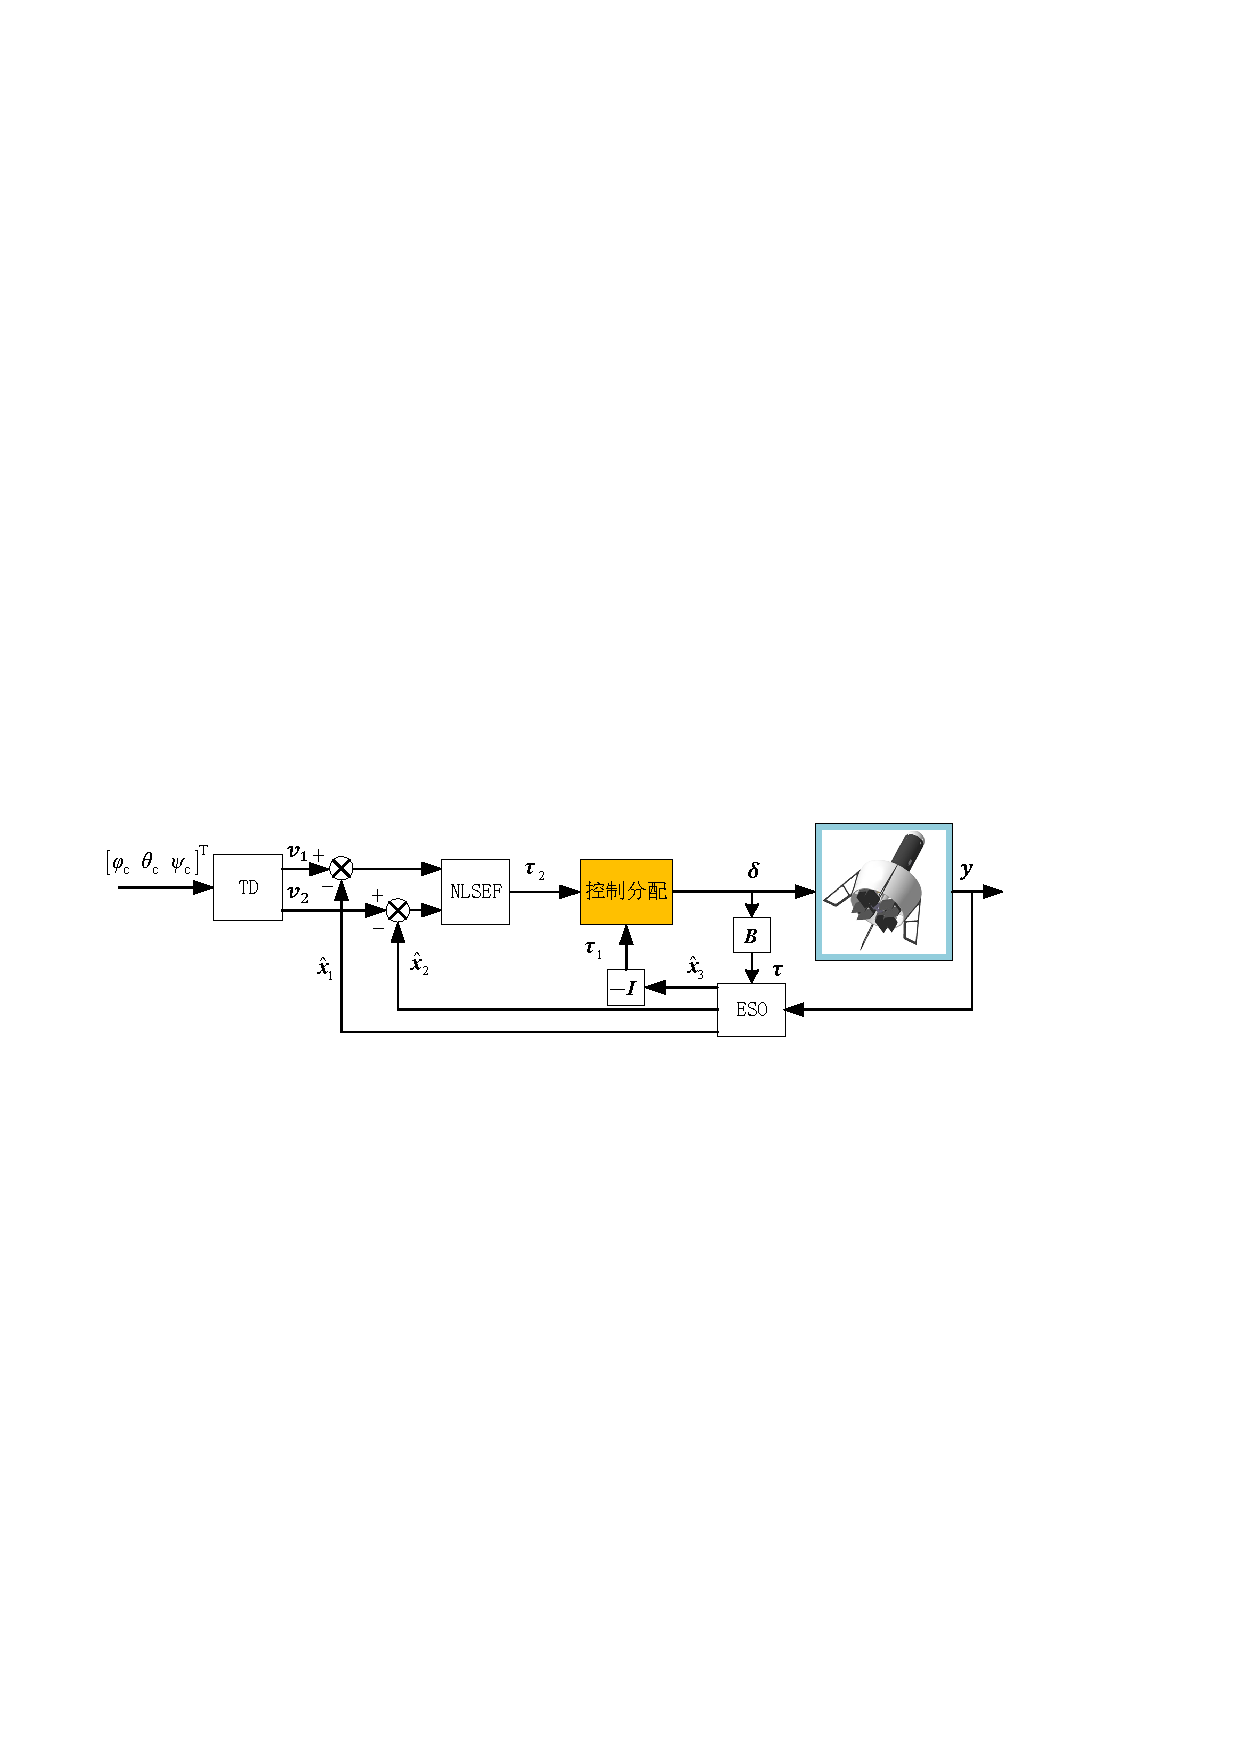
\includegraphics[scale=1]{Fig/prio_base_ADRC.pdf}
	\caption{\label{prio_base_ADRC}基于优先级控制分配单涵道姿态控制}
\end{figure}
\section{双涵道控制分配}
本节将介绍用于双涵道无人机的动态控制分配方法,并讨论其参数整定。由于双涵道将使用两种不同的执行器,执行器动力学和控制分配器之间的相互作用会导致实际执行的虚拟控制命令小于期望值。 为了补偿这种衰减,将使用后补偿方法来修改分配器的输出,而控制分配时仍忽略执行器动态。
\subsection{操纵面模型}
和单涵道不同,双涵道的滚转操纵面能提供的角加速度太小,以至于机动性太差,因而考虑将左右两个涵道风扇用来提供额外的滚转力矩。由式\eqref{eq_prop}、\eqref{eq_TDF_M_c},将驱动力矩重写为
\begin{align}
\bm{M}_{c}=
\begin{bmatrix}
-{{l}_{1}}\left(F_1-F_3+F_5-F_7\right) +(T_{La}-T_{Ra})l_2 \\
{{l}_{1}}\left(-F_2+F_4-F_6+F_8\right) \\
\left(l_3 F_{1} - l_4 F_{2} + l_3 F_{3} + l_5 F_{4} + l_3 F_5 + l_5 F_6 + l_3 F_7 + -l_4 F_8 \right)
\end{bmatrix}	\label{eq_new_TDF_M_c}
\end{align}	

分别记左、右涵道风扇转速为$ \varpi_{{1}} $、$ \varpi_{{2}} $,定义操纵面$\delta_9=\varpi_{{1}}-\varpi_{{2}}$,并定义 $\varpi _{{s}}=\varpi_{{1}}+\varpi_{{2}}$,有
\begin{align}
T_{Lp}- T_{Rp} = k_{\varpi}\left( \varpi _{{1}}^{2}-\varpi _{{2}}^{2} \right)= k_{\varpi} \varpi_{{s}}  \delta_9
\end{align}
此时,双管风扇无人机的操纵面是八个控制舵和风扇(将两个风扇当作一个操纵面使用)。 参照式\eqref{eq_tayler}的处理,得线性操纵面模型
\begin{gather}
\bm{\tau}=\bm{I}^{-1}\bm{M}_{ {c}}=\bm{B}\bm{\delta}	\\
\bm{B}\triangleq \bm{I}^{-1}\bm{P}diag\left( k_{\delta} (V_i+V_c)^2,\ldots ,k_{\delta} (V_i+V_c)^2, k_{\varpi}\varpi_s \right) \\
\bm{\delta}\triangleq {\left[ 
	\begin{matrix}
	\delta_1 & \delta_2 & \ldots  & \delta_8 & \delta_9  \\
	\end{matrix} \right]}^\top	\\
\bm{P} \triangleq \begin{bmatrix}
-l_{1} & 0 & l_{1} & 0 & -l_{1} & 0 & l_{1} & 0 & l_2\\
0 & -l_{1} & 0 & l_{1} & 0 & -l_{1} & 0 & l_{1}  &0\\
l_{3} & -l_{4} & l_{3} & l_{5} & l_{3} & l_{5} & l_{3} & -l_{4}&0 
\end{bmatrix}
\end{gather}

如前文所述,每个控制舵偏转角的范围是$\pm {{20}^{{}^\circ }}$,用弧度制表示即$\pm {\frac{\pi}{9}\, \text{rad}}$。驱动操纵面的执行器如图\ref{servo}所示,其最大转动角速率为$\frac{80\pi}{9}\, {\text{rad}}/{\text{s}}$。 涵道风扇由如图\ref{motor}所示的电机驱动,其转速范围为$300 \sim 1600\,{\text{rad}}/{\text{s}}\,$,转速变化率最大值为$800\,{\text{rad}}/{{{\text{s}}^{2}}}$。 在上文我们定义操纵面$\delta_9$代表左右涵道风扇的转速差, 考虑到风扇应主要用于提供升力,因此将用于提供滚转力矩的风扇转速范围限制为$-200 \sim 200\,{\text{rad}}/{\text{s}}\;$,因此有
\begin{gather}
\underline{\bm{\delta}}	=\left[ \begin{matrix}
-\dfrac{\pi}{9} & \cdots & -\dfrac{\pi}{9} & -200 
\end{matrix} \right]^\top	\\
\overline{\bm{\delta}} =\left[ \begin{matrix}
\dfrac{\pi}{9}  & \cdots   & \dfrac{\pi}{9} & 200  
\end{matrix} \right]^\top	\\
\bm{u}_{m}=\left[ \begin{matrix}
\dfrac{80\pi}{9}  & \cdots  & \dfrac{80\pi}{9}  & 800  
\end{matrix} \right]^\top	\label{eq_TDF_constraint}
\end{gather}
  
下面针对上述控制效率矩阵和操纵面约束,从两个方面分析双涵道控制分配的特点。

一方面,AMS的范围由位置约束和控制效率矩阵确定\cite{Durham_2017}。 在悬停点附近,测得双涵道无人机的控制效率矩阵为
\begin{align}\bm{B}=
\begin{bmatrix}
-4.67 & 0 & 4.67 & 0 & -4.67 & 0 & 4.67 & 0 & 0.08 \\
0 & -14.96 & 0 & 14.96 & 0 & -14.96 & 0 & 14.96 & 0 \\
4.26 & -6.96 & 4.26 & 15.49 & 4.26 & 15.49 & 4.26 & -6.96 & 0
\end{bmatrix}
\end{align}
根据上式和式\eqref{eq_TDF_constraint}绘制双涵道的AMS,如图\ref {TDF_AMS}所示。图\ref {TDF_AMS}还给出了伪逆方法的可达集,其品质因数仅为$16.96\%$,和单涵道的分析类似,伪逆法使操纵面牺牲了大量的潜在性能,因此需要一种更有效的方法。
\begin{figure}[htb]
	\centering
	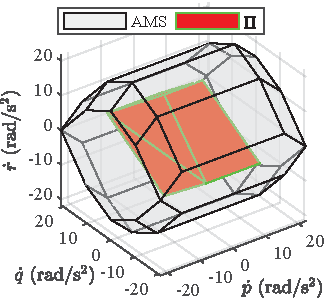
\includegraphics[scale=1]{Fig/TDF_AMS.pdf}
	\caption{\label{TDF_AMS}双涵道的AMS和伪逆法可达集$\Pi$}
\end{figure}

另一方面,由于使用了两种不同带宽的执行器,因此需要考虑执行器动力学的影响。 双涵道的执行器是如图\ref{servo}、图\ref{motor}所示的数字舵机和无刷直流电机。 其中电机的带宽小于数字舵机的带宽,分配器输出的执行器指令经过执行器环节后实际操纵面偏转角会产生明显的衰减\cite{Harkegaard_2004}。 根据$ \bm{\delta} $的位置限制,控制舵产生的滚转力矩范围小于涵道风扇,而且控制舵还产生气动阻力\cite{Speck_2013a}。 因此,希望尽可能避免使用控制舵产生滚转力矩。本文考虑根据执行器的带宽分配不同频率的伪控制输入,并补偿由执行器动态引起的衰减。
\begin{figure}[htbp]
	\centering
	\begin{minipage}[c]{0.5\textwidth}
		\centering
		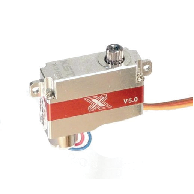
\includegraphics[scale=1.3]{Fig/servo.pdf}
	\end{minipage}%
	\begin{minipage}[c]{0.5\textwidth}
		\centering
		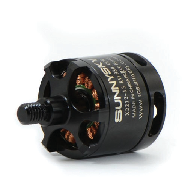
\includegraphics[scale=1.3]{Fig/motor.pdf}
	\end{minipage}\\[1pt]
	\begin{minipage}[t]{.5\textwidth}
		\caption{\label{servo}数字舵机}
	\end{minipage}%
	\begin{minipage}[t]{.5\textwidth}
		\caption{\label{motor}无刷直流电机}
	\end{minipage}%
\end{figure}
\subsection{动态控制分配}
在第二章中介绍了加权最小二乘控制分配,动态控制分配可看作是WLS法的推广。回顾控制分配问题表述:给定伪控制输入$\bm{\tau}={{\bm{\tau}}_{ {c}}}-\bm{\eta }$,求$\bm{\delta} \in \Omega$,使得 $\bm{\tau}=\bm{B}\bm{\delta}$,若有多个解,选择最优解;若没有解决方案,则寻求一个使分配误差$\bm{v }-\bm{B}\bm{u}$最小的解$\bm{\delta} \in \Omega$。 注意到,在双涵道的操纵面模型中,截距项$ \bm{\eta }=\bm{0} $。

在WLS方法的最优化指标中加入一项速度惩罚项,可得如下最优分配
\begin{gather}
{\bm{\delta}_{{\text{dca}}}} = \mathop {{\text{argmin}}}\limits_{\bm{\delta} \in \Theta }\; l\left( {\bm{\delta},\bm{v}} \right) \label{eq_sulotion_dca}	\\
l\left( {\bm{\delta},{\bm{v}_{{c}}}} \right) \triangleq 
\gamma {\left\| {{\bm{W}_{{v}}}\left( {\bm{v} - \bm{B\delta}} \right)} \right\|^2} + 
{\left\| {{\bm{W}_1}\left( {\bm{\delta} - {\bm{\delta}_{{s}}}} \right)} \right\|^2} + 
{\left\| {{\bm{W}_2}\left( {\bm{\delta} - {\bm{\delta}_{{0}}}} \right)} \right\|^2} \label{29}
\end{gather}
%而$\left\|\,\centerdot\,\right\|$表示由$\left\| \bm{\delta} \right\|=\sqrt{{{\bm{\delta}}^{ {T}}}\bm{\delta}}$定义的范数,
其中${{\bm{\delta}}_{ {s}}}$是期望的稳态控制输入,${{\bm{\delta}}_{0}}$是上一采样时刻的控制输入, ${{\bm{W}}_{1}}$、${{\bm{W}}_{2}}$和${{\bm{W}}_{ {v}}}$ 是加权矩阵。 类似WLS法,加权因子$ \gamma $应该是一个大的标量值。

因此,如果问题没有解,则矩阵${{\bm{W}}_{ {v}}}$ 将加权分配误差来影响伪控制输入的限幅方式。如果问题有多个解,则矩阵${{\bm{W}}_{1}}$ 和 ${{\bm{W}}_{2}}$将平衡跟踪 ${{\bm{u}}_{ {s}}}$ 和 ${{\bm{u}}_{0}}$ 。${{\bm{W}}_{1}}$的需求,矩阵${{\bm{W}}_{1}}$的对角线元素越大,相应的执行器收敛越快,${{\bm{W}}_{2}}$ 的对角线元素越大,将使执行器指令变化幅度越小。如果满足以下假设,则式\eqref {eq_sulotion_dca}是唯一的最优解\cite{Harkegaard_2004}
\begin{assumption}
加权矩阵${{\bm{W}}_{1}}$和 ${{\bm{W}}_{2}}$ 是对称矩阵,且$ {{\bm{W}}_{2}}$非奇异。	\label{assum_dca1}
\end{assumption}

为了确定参数${{\bm{u}}_{ {s}}}$,$\bm{W}_1$和$\bm{W}_2$,我们首先讨论式\eqref{eq_no_constraint_problem}所示的无约束控制分配问题的解,并陈述以下定理而无需证明\cite{Harkegaard_2004}。
\begin{alignat}{2}
\begin{split}
\mathop {{\text{min}}}\limits_{\bm{\delta} }\quad& {\left\| {{\bm{W}_1}\left( {\bm{\delta} - {\bm{\delta}_{{s}}}} \right)} \right\|^2} + 
{\left\| {{\bm{W}_2}\left( {\bm{\delta} - {\bm{\delta}_{{0}}}} \right)} \right\|^2}\\
\mbox{s.t.}\quad
&\bm{v }=\bm{B}\bm{\delta} 
\end{split} \label{eq_no_constraint_problem}
\end{alignat}

\begin{theorem}
	如果假设\ref{assum_dca1}成立,则问题\eqref{eq_no_constraint_problem}有解
	\begin{align}
	\bm{\delta} = \bm{E}{\bm{\delta}_{{s}}} + \bm{F}{\bm{\delta}_{{0}}} + \bm{Gv} \label{eq_solution_no_constraint_problem}
	\end{align}
	其中
	\begin{align}
	\bm{E} &=\left( \bm{I}-\bm{GB} \right){{\bm{W}}^{-2}}\bm{W}_{1}^{2}\\
	\bm{F} &=\left( \bm{I}-\bm{GB} \right){{\bm{W}}^{-2}}\bm{W}_{2}^{2}	\label{eq_F} \\
	\bm{G} &=\left( \bm{B}{{\bm{W}}^{-1}} \right)^{+}
	\end{align}
	且加号逆即伪逆定义为$ 	{{\bm{B}}^{+}}={{\bm{B}}^{{T}}}{{\left( \bm{B}{{\bm{B}}^{{T}}} \right)}^{-1}} $。	\label{the_dca1}
\end{theorem}
\begin{theorem}
	如果假设\ref{assum_dca1}成立,$\bm{F}$满足式\eqref{eq_F}的定义,且${{\bm{W}}_{1}}$非奇异,则有$0\le e \left( \bm{F} \right) < 1$,其中$e \left( \bm{F} \right)$是 $\bm{F}$的特征值。	\label{the_dca2}
\end{theorem}
\begin{theorem}
	若矩阵${{\bm{W}}_{1}}$非奇异,且$\bm{\delta}_{ {s}}$满足等式$\bm{B}\bm{\delta}_{ {s}}=\bm{v}$,那么对式\eqref {eq_no_constraint_problem}中的$\bm{\delta}_{ {s}}$,有$\underset{t\to \infty }{\mathop{\lim }}\,\bm{\delta}\left( t \right)={{\bm{\delta}}_{ {s}}}$。	\label{the_dca3}
\end{theorem}

定理\ref{the_dca1}表明\eqref{eq_no_constraint_problem}的解由\eqref{eq_solution_no_constraint_problem}给出,这是一个线性滤波器。 该滤波器的极点是$\bm{F}$的特征值。 定理\ref{the_dca2}表明,如果${{\bm{W}}_{1}}$是非奇数,则\eqref{eq_solution_no_constraint_problem}是渐近稳定的。 定理\ref{the_dca3}则表明,如果$\bm{\delta}_{ {s}}$是一个容许控制,则它将最终收敛到该值上。

在研究的无人机中,伪控制输入 $\bm{\tau}$ 和期望的稳态输入 ${{\bm{\delta}}_{ {s}}}$的每个组成部分都同样重要,因此 ${{\bm{W}}_{ {v}}}$和${{\bm{W}}_{1}}$可分别取为相应维数的单位矩阵。${{\bm{W}}_{2}}$ 的对角线项是相应执行器的速度惩罚因子。 由于低带宽执行器应将其驱动的操纵面尽可能保持为${{\bm{ \delta}}_{0}}$中对应值,因此低带宽执行器对应的惩罚因子应大于高带宽执行器。 在该设置下,慢速执行器主要用于产生低频伪控制输入,而高频伪控制输入主要分配给高带宽执行器。 

${{\bm{ \delta}}_{ {s}}}$可以取为以下优化问题的解
\begin{alignat}{2}
\begin{split}
\mathop {{\text{min}}}\limits_{\bm{ \delta} }\quad&{\left\| {{\bm{W}_{ {s}}}\left( {{\bm{ \delta}_{ {s}}} - {\bm{ \delta}_{ {d}}}} \right)} \right\|^2} \\
\mbox{s.t.}\quad
&\bm{v }=\bm{B}\bm{ \delta}_{ {s}}
\end{split} \label{eq_solu_u_s}
\end{alignat}
其中首选值 ${{\bm{ \delta}}_{ {d}}}$ 通常取为满足特定要求但不在容许控制集内的固定值。 为了使控制舵在稳态时的气动阻力最小,选择${{\bm{ \delta}}_{ {d}}}={{\bm{0}}_{9\times 1}}$和 ${{\bm{W}}_{ {s}}}\bm{=I}$,即取${{\bm{ \delta}}_{ {s}}}$为某种广义逆解。

为了确保控制舵有一定的余量来处理可能的高频伪控制输入,进入稳定状态后,滚转相关的控制舵应保持零偏转。 因此,考虑将$ \bm{ \delta}_{ {s}} $的分量的约束${ \delta_{ {s},\, {i}}}=0$, $i=1,3,5,7$添加到\eqref{eq_solu_u_s}中,则其解可以通过以下方法获得:将控制有效性矩阵$\bm{B}$分为${{\bm{B}}_{1}}$和${{\bm{B}}_{2}}$,其中${{\bm{B}}_{1}}$由与滚转相关的控制舵对应的$\bm{B}$列组成,${{\bm{B}}_{2}}$为其余的列组成。对$\bm{B}$的广义逆矩阵$\bm{S}$进行类似的矩阵分块,使得$\bm{I} ={\bm{B}_1}{\bm{S}_1} + {\bm{B}_2}{\bm{S}_2}$。 取${{\bm{S}}_{1}}={{\bm{0}}_{4\times 9}}$和${{\bm{S}}_{2}}=\bm{B}_{2}^{+}$,因此,式\eqref{eq_solu_u_s}的解可以取为${{\bm{ \delta}}_{ {s}}}=\bm{S}\bm{v}$。 至此,可以通过二次规划方法来求解动态控制分配问题的解\eqref {eq_sulotion_dca},例如有效集方法。
\subsection{补偿执行器动态}
到目前为止,在讨论双涵道的控制分配时都假定$ \bm{\delta} = \bm{ \delta}_c $。 然而,如前文所述,在双涵道中,执行器的动力学不可忽略。上文中动态控制分配求得的解实际上是执行器指令$ \bm{\delta}_c $,而实际执行器输出即操纵面偏转角为$ \bm{\delta} $。对双涵道使用的数字舵机和无刷直流电机,其执行器动力学模型式\eqref{eq_atuacor}可近似用一阶微分方程表示。设某个执行器环节的传递函数为
\begin{align}
\frac{\delta_{ {i}}\left( s \right)}
{ \delta_{c {i}}\left( s\right)}
=\frac{a_i}{s+a_{ {i}}}
\end{align}
其中$ i=1,2,\ldots,9 $,$ a_i $为执行器带宽。上式对应的离散化状态方程为
\begin{align}
\delta_{ {i}}\left( k+1 \right)=A_{ {i}}  \delta _{ {i}} \left( k \right)+H_{ {i}}  \delta_{c {i}}\left( k \right) \label{14}
\end{align}
其中$A_{ {i}}\triangleq {e}^{ {-{{a}_{i}}T}}$,$H_{ {i}}\triangleq 1-{e}^{ {-{{a}_{i}}T}}$,$ T $为系统控制周期,执行器指令$ \delta_{c {i}}\left( k \right)$通常在每个控制周期内保持恒定,将输入重写为
\begin{align}
 \delta_{c {i}}\left( k \right)= \Delta  \delta_{ci}\left( k \right)+ \delta _{ {i}}\left( k \right) \label{15}
\end{align}
其中$\Delta  \delta_{c {i}}\left( k \right)= \delta_{ c{i}}\left( k \right)-\delta _{ {i}}\left( k \right)$,可将其视为执行器的阶跃输入。 $ \delta_{c {i}}\left( k \right)$由忽略执行器动态求解得到的动态控制分配的解。 将\eqref{15}带入为\eqref{14}可得
\begin{align}
\begin{split}
\delta_{ {i}}\left( k+1 \right) &=A_{ {i}}  \delta _{ {i}} \left( k \right)+H_{ {i}} \left(\Delta  \delta_{ c{i}}\left( k \right)+ \delta _{ {i}}\left( k \right) \right)=H_{ {i}}\Delta  \delta_{c {i}}\left( k \right)+\delta _{ {i}}\left( k \right) 
\end{split}
\end{align}
其中$H_{ {i}}<1$,执行器指令的增量$\Delta  \delta_{c {i}}\left( k \right)$经过执行器环节后产生了衰减,因此$\delta_{ {i}}\left( k+1 \right) \neq  \delta_{ c{i}}\left( k \right)$。

考虑寻找增益$K_{ {i}}$来修改执行器指令增量,使$\delta_{ {i}}\left( k+1 \right) =  \delta_{ c{i}}\left( k \right)$,因此$\delta_{ {i}}\left( k+1 \right) =A_{ {i}}  \delta _{ {i}} \left( k \right)+H_{ {i}} \left(K_{ {i}} \Delta  \delta_{ c{i}}\left( k \right)+ \delta _{ {i}} \left( k \right) \right) =   \delta_{c {i}}\left( k \right)
$,因而有
\begin{gather}
K_{ {i}} = {H_{ {i}}}^{-1} \\
\hat{ \delta}_{c {i}}\left( k \right) = \left(K_{ {i}} \Delta  \delta_{c {i}}\left( k \right)+ \delta _{ {i}} \left( k \right) \right)
\end{gather}
其中$K_{ {i}}$是补偿增益,$\hat{ \delta}_{ c{i}}\left( k \right)$是修改后的执行器命令。

\begin{figure}[tbp]
	\centering	
	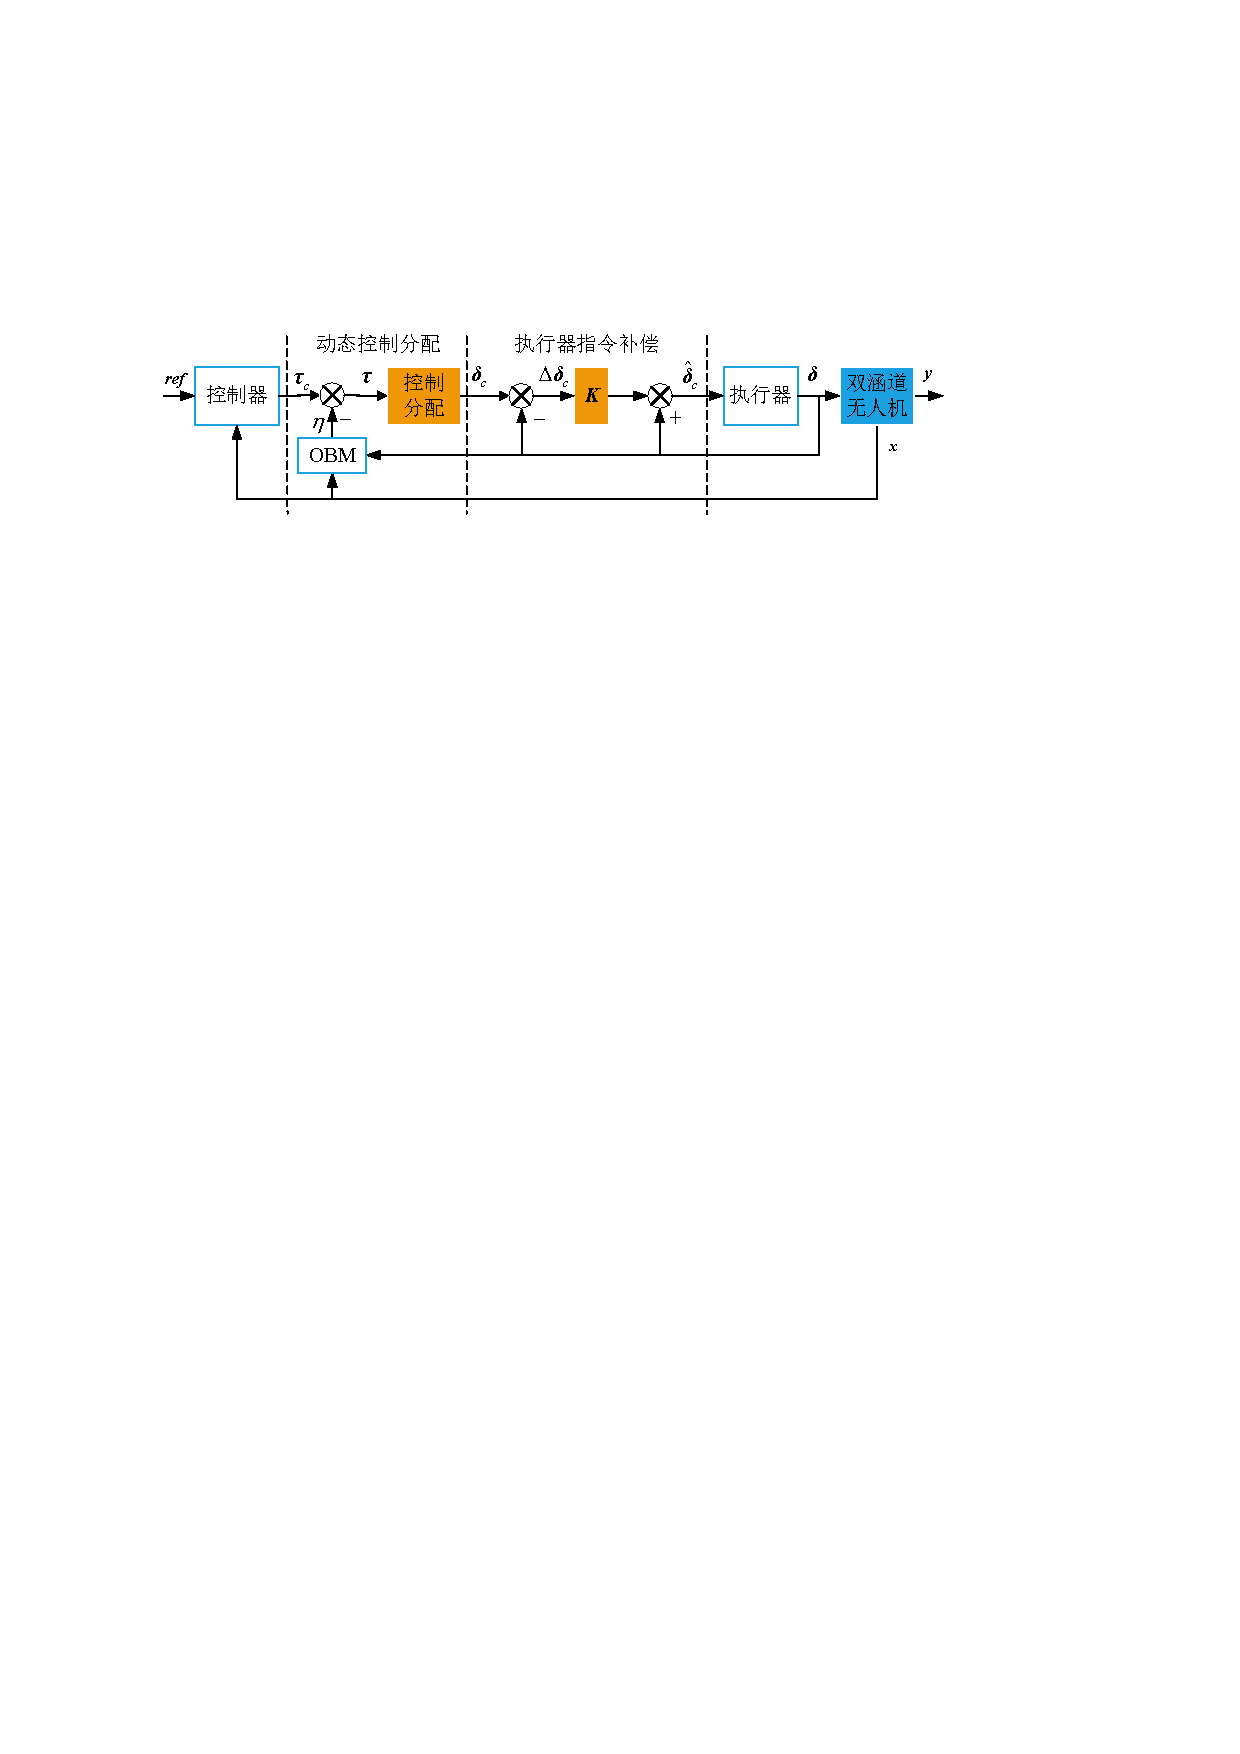
\includegraphics[scale=1]{Fig/TDF_allocation.pdf}
	\caption{\label{allocation}含执行器动态补偿的双涵道控制分配}
\end{figure}

在实现中,$H_{ {i}}$可以用标称带宽$a_{ {i,nom}}$计算其近似值,$a_{ {i,nom}}$是实际带宽的上限,因此可以通过补偿控制分配器输出来减小执行器动态的影响\cite{Oppenheimer_2004}。 对于一组独立的一阶执行器,包含执行器指令增量补偿的控制分配如图\ref{allocation}所示,其中补偿增益取为$\bm{K} = diag\left( K_1,K_2,\ldots,K_{ {p}} \right)$,OBM为用于计算截距项的机载系统模型。 
%
\section{本章小结}
%
伪控制输入其维数通常等于系统自由度,在线性操纵面模型下,可达的伪控制输入是容许控制经控制效率矩阵线性$ \bm{B} $映射得到,此时过驱动系统的控制分配问题是由于控制向量的维数大于伪控制输入维数引起的。求解控制分配问题就是给定伪控制输入,求$ \bm{B} $的逆映射。引入控制分配环节后,控制系统可分层设计。本章基于分层设计的方法讨论了两种涵道风扇式无人机的控制分配问题及其解法。

对于单涵道,提出一种优先级控制分配方法,该方法先将期望力矩进行矢量分解,并按一定优先级排序,对该优先级序列引入比例因子求解约束最优化问题,使得高优先级分量尽可能无误差分配。当期望力矩可达时,该方法等价于直接分配法,当期望力矩不可达时,该方法引入的比例因子对期望力矩的低优先级分量进行放缩,相当于截断低优先级分量,保证高优先级分量无分配误差。将该方法应用于到基于ADRC进行姿态控制的单涵道控制系统上,可减小执行器饱和的几率,并在一定程度上避免输出耦合。

对于双涵道,利用两个涵道风扇产生的升力提供额外的滚转力矩,扩大了其可达集范围。由于使用了不同带宽的执行器,本章利用了动态控制分配方法求解其控制分配问题,并对执行器动态进行补偿。


%类似单涵道的处理,将双涵道的驱动力矩式\eqref{eq_TDF_M_c}改写为
%\begin{align}
%\bm{M}_{c}=\begin{bmatrix} \tau_{x} \\ \tau_{y} \\ \tau_{z} \end{bmatrix}=\begin{bmatrix}
%-l_{1} & 0 & l_{1} & 0 & -l_{1} & 0 & l_{1} & 0 \\
%0 & -l_{1} & 0 & l_{1} & 0 & -l_{1} & 0 & l_{1}  \\
%l_{3} & -l_{4} & l_{3} & l_{5} & l_{3} & l_{5} & l_{3} & -l_{4} 
%\end{bmatrix} k_{\delta} (V_i+V_c) \bm{\delta}
%\end{align}
%其中$\bm{\delta } = [\delta_1 \quad \delta_2 \quad \ldots \quad \delta_8]^\top$。由表\ref{TDF_para}可知,双涵道不同通道的转动惯量差别较大,为了使可达集更直观和无人机机动性能相关,考虑取角加速度为伪控制指令,即
%\begin{align}
%\bm{\tau}=\bm{I}^{-1}\bm{M}_{ {cs}}=\bm{B}\bm{\delta}
%\end{align}
%并仍称$ \bm{\tau} $为力矩,其中控制效率矩阵为
%\begin{align}
%\bm{B}=\bm{I}^{-1}\begin{bmatrix}
%-l_{1} & 0 & l_{1} & 0 & -l_{1} & 0 & l_{1} & 0 \\
%0 & -l_{1} & 0 & l_{1} & 0 & -l_{1} & 0 & l_{1}  \\
%l_{3} & -l_{4} & l_{3} & l_{5} & l_{3} & l_{5} & l_{3} & -l_{4} 
%\end{bmatrix} k_{\delta} (V_i+V_c)
%\end{align}
%结合操纵面幅值约束
%\begin{align}
%\bm{u}_{ {min}}	&=\left[ \begin{matrix}
%-{\pi }/{9} & \cdots & -{\pi }/{9} & -200 
%\end{matrix} \right]^{ {T}}	\\
%\bm{u}_{ {max}} &=\left[ \begin{matrix}
%{\pi }/{9}  & \cdots   & {\pi }/{9} & 200  
%\end{matrix} \right]^{ {T}}
%\end{align}
%绘制其AMS如图所示。可见滚转通道由于转动惯量太大而导致可达的角加速度太小。为解决这个问题,需要将左右涵道的风扇用来提供滚转力矩。






%\begin{gather}
%\bm{M}_{{cs}}=\bm{P} \bm{F} \\
%\bm{P} \triangleq\left[\begin{array}{ccccccccc}
%-l_{1} & 0 & l_{1} & 0 & -l_{1} & 0 & l_{1} & 0 & l_{2} \\
%0 & -l_{1} & 0 & l_{1} & 0 & -l_{1} & 0 & l_{1} & 0 \\
%l_{3} & -l_{4} & l_{3} & l_{5} & l_{3} & l_{5} & l_{3} & -l_{4} & 0
%\end{array}\right] \\
%\bm{F} \triangleq\left[F_{1} \quad F_{2} \quad \ldots \quad  F_{9}\right]^\top \label{19}
%\end{gather}
%其中 $\bm{P}$是力矩臂矩阵,$F_{ {k}}$, $k=1,2,\ldots ,8$是控制叶片产生的气动升力,$F_{ {9}}$是两个风管风扇之间的升力差。\eqref{19}中的力可以表示为
%\begin{align}
%{{F}_{ {k}}} &={{k}_{ {u}}}V_{ {\infty} }^{2}{{u}_{ {k}}},\quad k=1,2,\ldots ,8 \label{20}\\
%T_{ {j}} &=k_{ {t}}\varpi _{ {j}}^{2},\quad j=1,2 \label{21}
%\end{align}
















